% LuaLaTeX文書; 文字コードはUTF-8
\documentclass[unicode,12pt]{beamer}% 'unicode'が必要
\usepackage{luatexja}% 日本語したい
\usepackage[ipaex]{luatexja-preset}% IPAexフォントしたい
\renewcommand{\kanjifamilydefault}{\gtdefault}% 既定をゴシック体に

\usepackage{amssymb,amsmath,ascmac}
\usepackage{derivative}

\usepackage{multirow}
\usepackage{bm}

\graphicspath{{../fig/}}
\usepackage[outdir=./]{epstopdf}

\usepackage{tikz}
\usepackage{xparse}



\usetikzlibrary{shapes,arrows}
%% define fancy arrow. \tikzfancyarrow[<option>]{<text>}. ex: \tikzfancyarrow[fill=red!5]{hoge}
\tikzset{arrowstyle/.style n args={2}{inner ysep=0.1ex, inner xsep=0.5em, minimum height=2em, draw=#2, fill=black!20, font=\sffamily\bfseries, single arrow, single arrow head extend=0.4em, #1,}}
\NewDocumentCommand{\tikzfancyarrow}{O{fill=black!20} O{none}  m}{
\tikz[baseline=-0.5ex]\node [arrowstyle={#1}{#2}] {#3 \mathstrut};}

%目次スライド
\AtBeginSection[]{
  \frame{\tableofcontents[currentsection]}
}
%アペンディックスのページ番号除去
\newcommand{\backupbegin}{
\newcounter{framenumberappendix}
\setcounter{framenumberappendix}{\value{framenumber}}
}
\newcommand{\backupend}{
\addtocounter{framenumberappendix}{-\value{framenumber}}
\addtocounter{framenumber}{\value{framenumberappendix}} 
}

%%%%%%%%%%%  theme  %%%%%%%%%%%
\usetheme{Copenhagen}
% \usetheme{Metropolis}
% \usetheme{CambridgeUS}
% \usetheme{Berlin}

%%%%%%%%%%%  inner theme  %%%%%%%%%%%
% \useinnertheme{default}

% %%%%%%%%%%%  outer theme  %%%%%%%%%%%
\useoutertheme{default}
% \useoutertheme{infolines}

%%%%%%%%%%%  color theme  %%%%%%%%%%%
%\usecolortheme{structure}

%%%%%%%%%%%  font theme  %%%%%%%%%%%
\usefonttheme{professionalfonts}
%\usefonttheme{default}

%%%%%%%%%%%  degree of transparency  %%%%%%%%%%%
%\setbeamercovered{transparent=30}

% \setbeamertemplate{items}[default]

%%%%%%%%%%%  numbering  %%%%%%%%%%%
% \setbeamertemplate{numbered}
\setbeamertemplate{navigation symbols}{}
\setbeamertemplate{footline}[frame number]

\title{粘着剤の基礎知識と評価法}
\subtitle{~ 第七章 東亞合成での開発例 ~}
\author[SDL Inc. 佐々木]{佐々木 裕\thanks{hsasaki@softmatters.net}}
\institute[]{元 東亞合成株式会社\\ソフトマターデザインラボ合同会社}
\date{2024/6/24}

\begin{document}

%%%%%
% 1 P
%%%%%
\maketitle

\begin{frame} 
    \tableofcontents[]
\end{frame} 

\section{高温連続ラジカル重合によるオリゴマー}
\subsection{東亞合成でのアクリル系材料}
\begin{frame}
	\frametitle{東亞合成でのオリゴマー}
		弊社では以前よりアクリル系ポリマーを利用した材料の開発を行ってきており、アクリル系オリゴマーの低価格製造法も確立してきている。

		\begin{block}{アクリル系オリゴマーの低価格製造法}
		\begin{itemize}
		\item 高温での連鎖移動を積極的に利用した塊状連続重合
		\item アクリル系モノマーを加熱された反応器へ連続的に供給
		\item オリゴマーを合成するプロセス
		\item 官能基を有するモノマーを共重合し反応性を付与可能
		\end{itemize}
		\end{block}
\end{frame}

\begin{frame}\frametitle{アクリル系モノマー}
\begin{figure}[!b]
	\begin{center}
		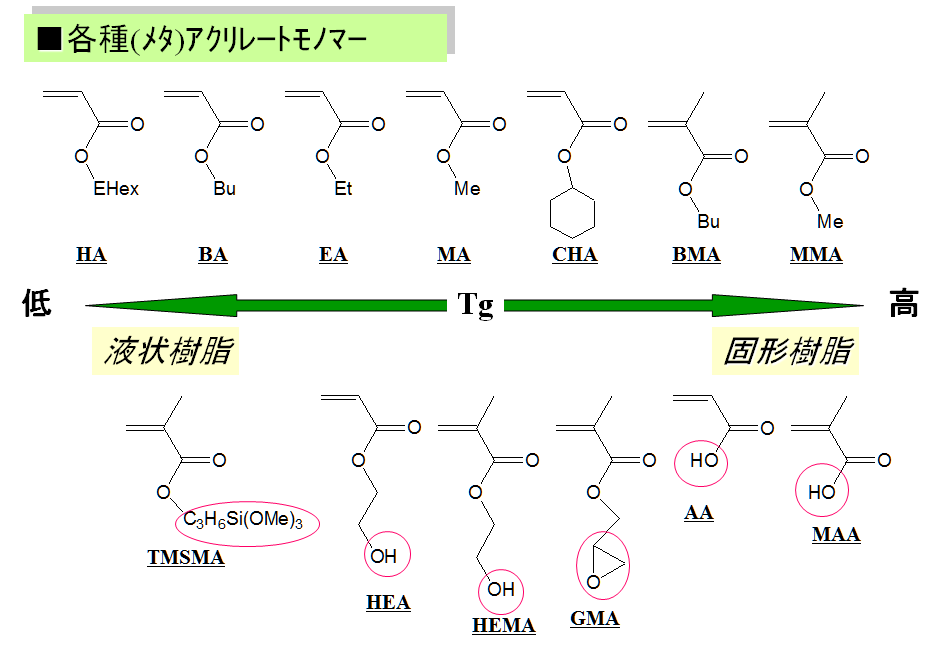
\includegraphics[width=100mm]{monomers.png}
	\end{center}
\end{figure}
\end{frame}

%%%%
\subsection{各種重合法と生成ポリマーの分子量}

\begin{frame}\frametitle{各種重合法と生成ポリマーの分子量}
\begin{figure}[!b]
	\begin{center}
		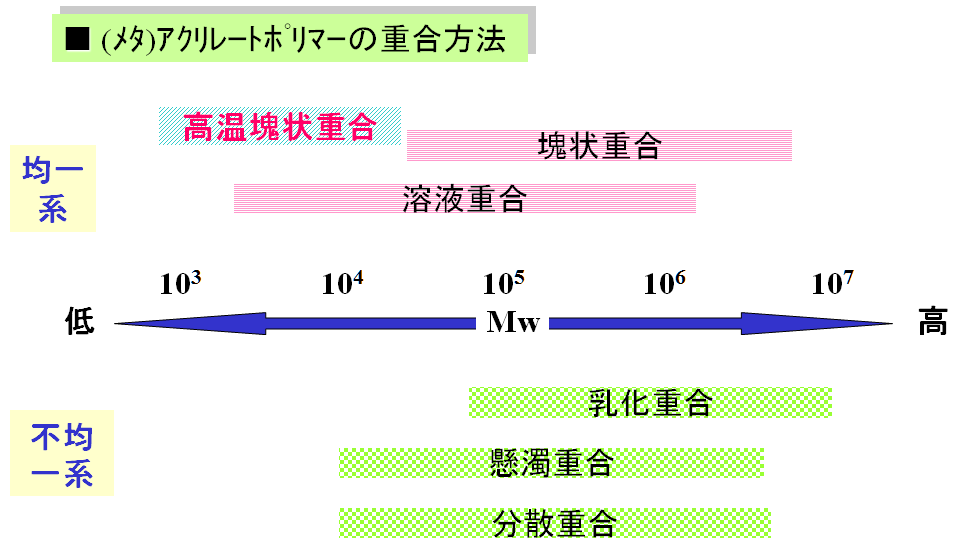
\includegraphics[width=100mm]{jyuugou_hou.png}
	\end{center}
\end{figure}
\end{frame}

\subsection{高温連続ラジカル重合について}
\begin{frame}\frametitle{高温連続ラジカル重合プロセス}
\begin{figure}[!b]
	\begin{center}
		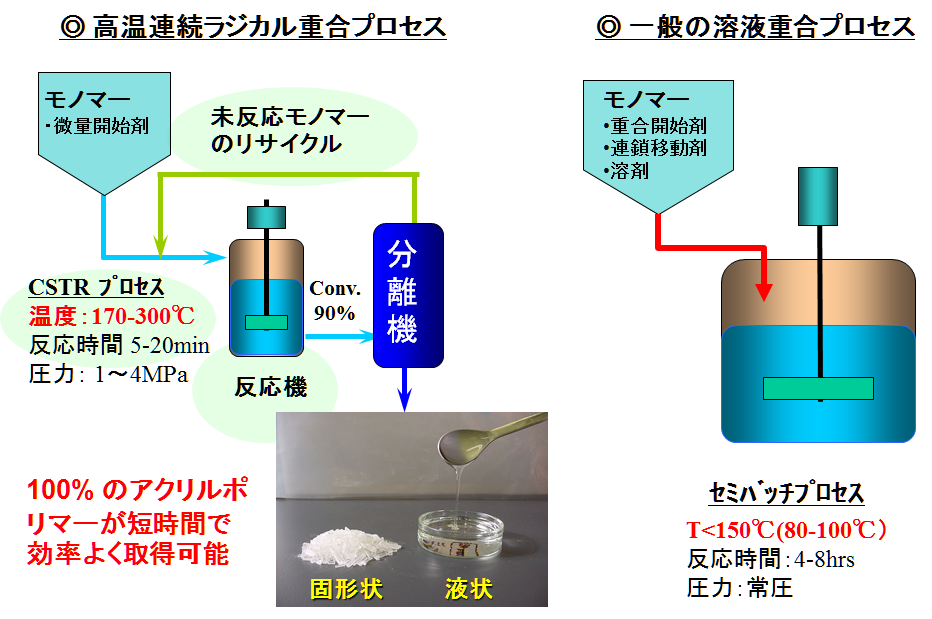
\includegraphics[width=100mm]{hikaku.png}
	\end{center}
\end{figure}
\end{frame}

%%%%%

%
\begin{frame}
	\frametitle{高温連続ラジカル重合の特徴}
		\begin{figure}[!b]
			\begin{center}
				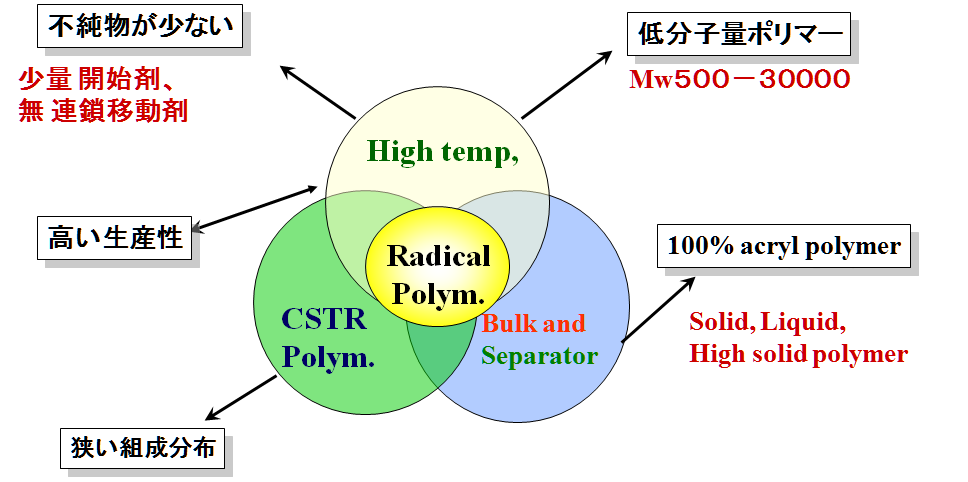
\includegraphics[width=100mm]{tokutyo.png}
			\end{center}
		\end{figure}
\end{frame}

%%%%%
%\section{高温ラジカル重合メカニズム}
%\subsection{高温ラジカル重合でのオリゴマー製造}
%
\begin{frame}
	\frametitle{高温ラジカル重合でのオリゴマー製造}
		\begin{figure}[!b]
			\begin{center}
				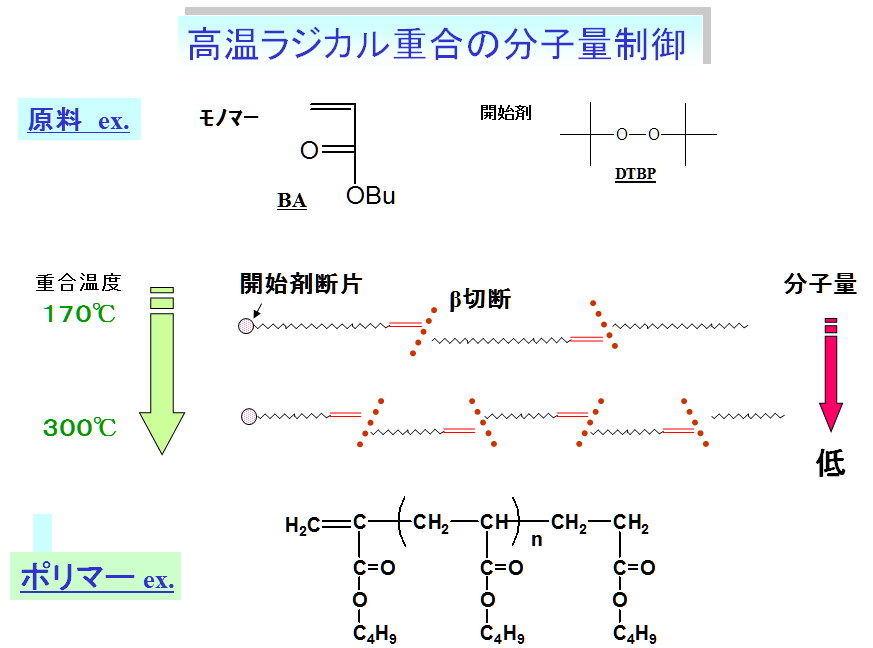
\includegraphics[width=90mm]{Mw_seigyo.png}
			\end{center}
		\end{figure}
		\end{frame}
		\begin{frame}\frametitle{オリゴマー製品}
		\begin{figure}[!b]
			\begin{center}
				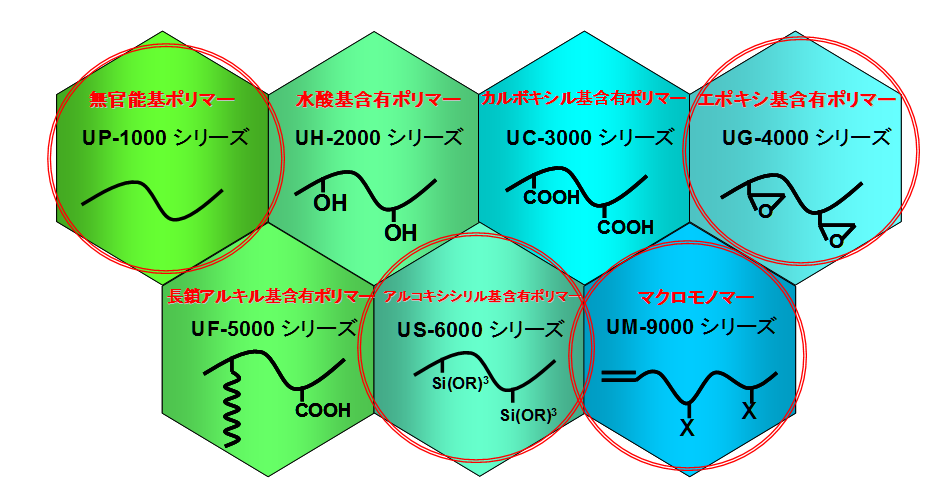
\includegraphics[width=100mm]{seihin.png}
			\end{center}
		\end{figure}
\end{frame}

\begin{frame}
	\frametitle{「高温連続ラジカル重合によるオリゴマー」のまとめ}
        \begin{boxnote}
            \vspace{-3mm}
            \begin{itemize}
                \item 東亞合成でのアクリル系材料
                    \begin{itemize}
                        \item アクリル系オリゴマーの低価格製造法も確立
                        \item 多様なモノマーを使用して各種の設計が可能
                    \end{itemize} 
                \item 各種重合法と生成ポリマーの分子量
                    \begin{itemize}
                        \item 重合法の選択により幅広い分子量のポリマー
                        \item 高温塊状重合を用いれば特徴あるオリゴマー
                    \end{itemize} 
                \item 高温連続ラジカル重合
                    \begin{itemize}
                        \item 無溶剤で液状オリゴマーが製造可能
                        \item 各種の特性を持った製品
                    \end{itemize}
            \end{itemize}
        \end{boxnote}
\end{frame}





%%%%%%%%%%%%%%%%%%%%%%%%%%%%%%%%%%%%%%%%%%%%%%%%%%%%%%%%%%%%%%%%%%%%%%%%%%%%%%%%%%%%%%%%%%%%%%%%%
\section{OCA改質用新規タッキファイヤーの開発}
\subsection{開発ターゲットの設定}
\begin{frame}
	\frametitle{OCA への要求性能}
	\begin{figure}
		\begin{center}
			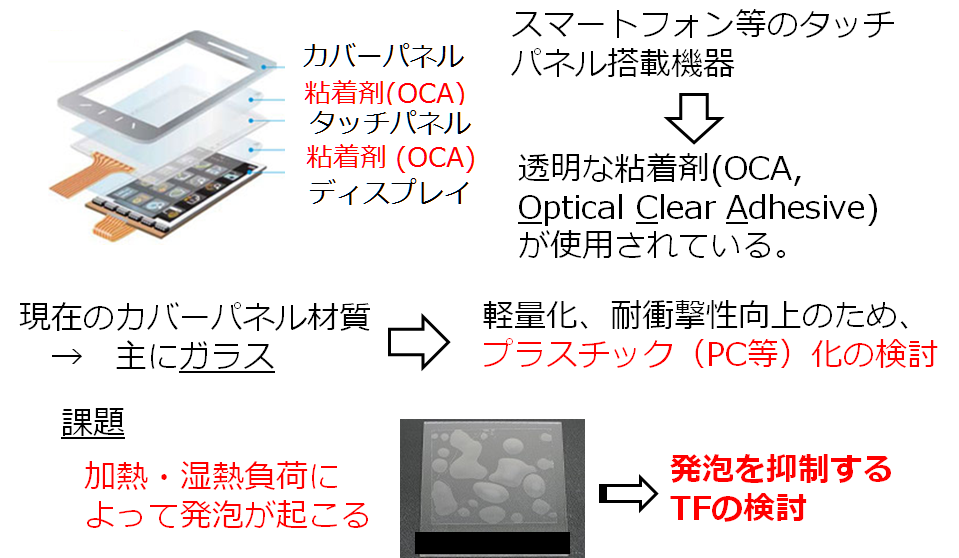
\includegraphics[width=100mm]{target.png}
		\end{center}
	\end{figure}
\end{frame}


%
\begin{frame}\frametitle{発泡現象とその機構の推定}
	\begin{figure}
		\begin{center}
			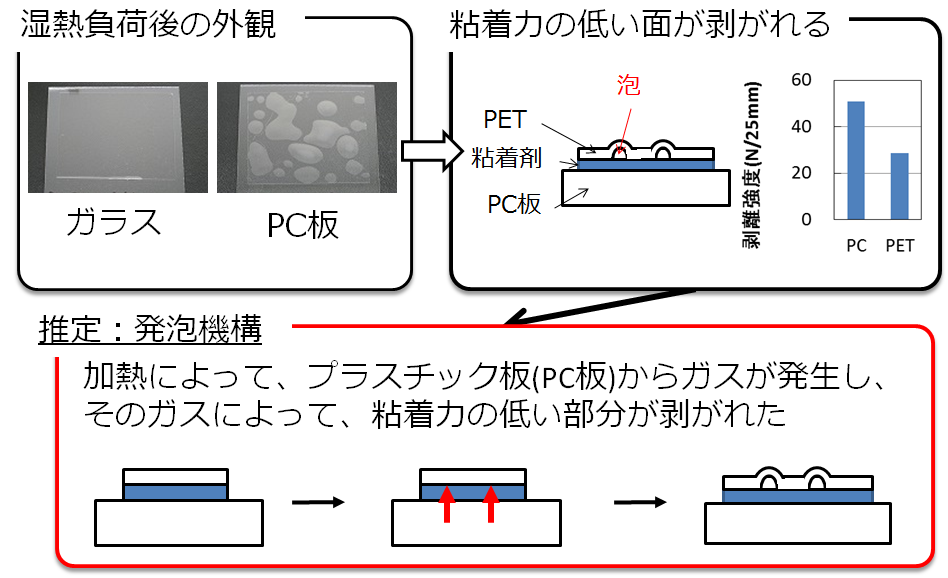
\includegraphics[width=100mm]{PC_delami.png}
		\end{center}
	\end{figure}
\end{frame}

\begin{frame}\frametitle{発泡抑制の考え方}
	\begin{figure}
		\begin{center}
			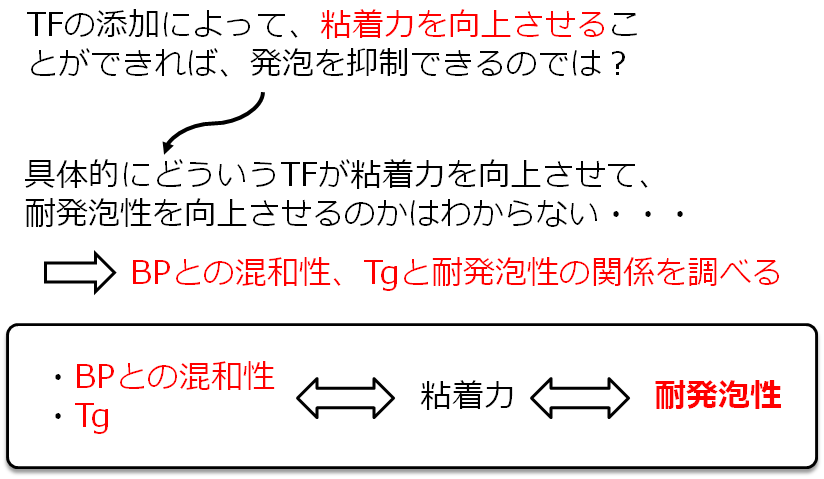
\includegraphics[width=100mm]{aproach.png}
		\end{center}
	\end{figure}
\end{frame}

%%%%%
\subsection{タッキファイヤーの選択}
%
\begin{frame}\frametitle{混和性と溶解度パラメータの関係}
	\begin{figure}
		\begin{center}
			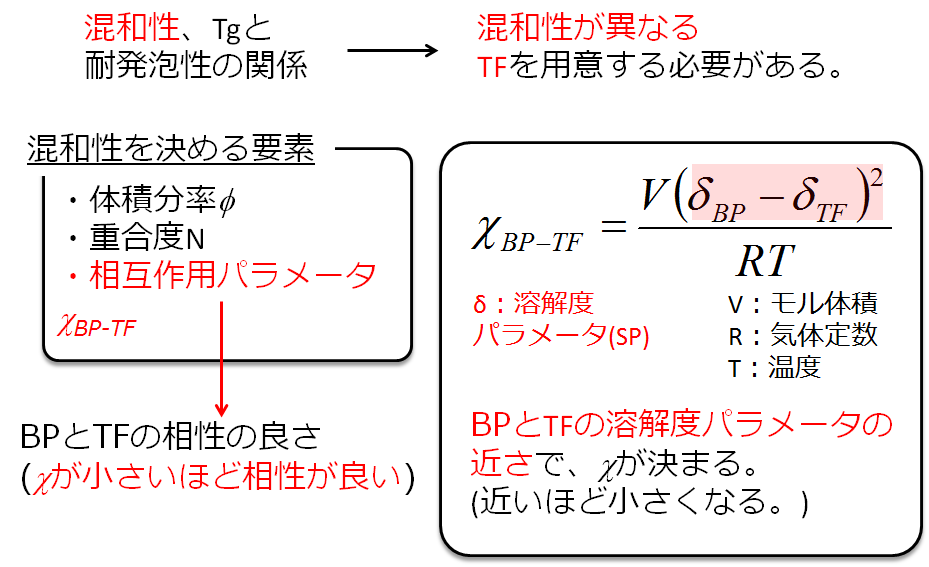
\includegraphics[width=100mm]{konwa.png}
		\end{center}
	\end{figure}
\end{frame}

\begin{frame}\frametitle{タッキファイヤーの SP 値}
	以下に示したように、SP 値(およびガラス転移温度	 Tg)の異なるタッキファイヤーを各種合成した。
		\begin{figure}
			\begin{center}
				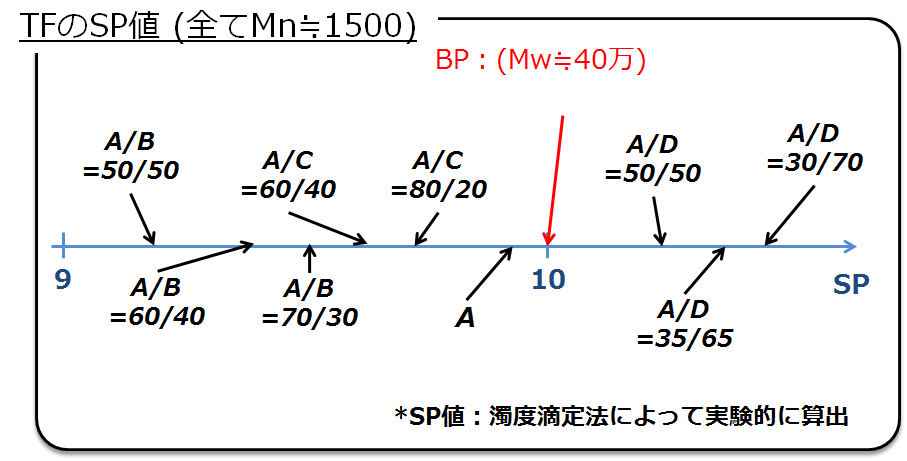
\includegraphics[width=100mm]{Tackifier_list.png}
			\end{center}
		\end{figure}
	\end{frame}
	
	%%%%%
	%
\begin{frame}\frametitle{混和性の評価方法}
	\begin{figure}
		\begin{center}
			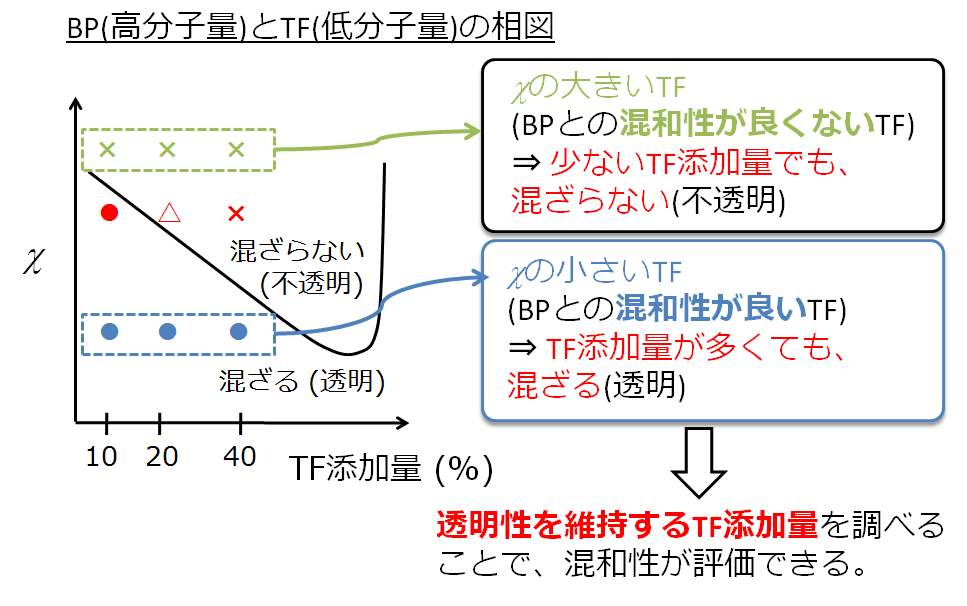
\includegraphics[width=100mm]{kanngaekata.png}
		\end{center}
	\end{figure}
\end{frame}

%%%%%
%
\begin{frame}\frametitle{相図による混和性の確認}
	\begin{figure}
		\begin{center}
			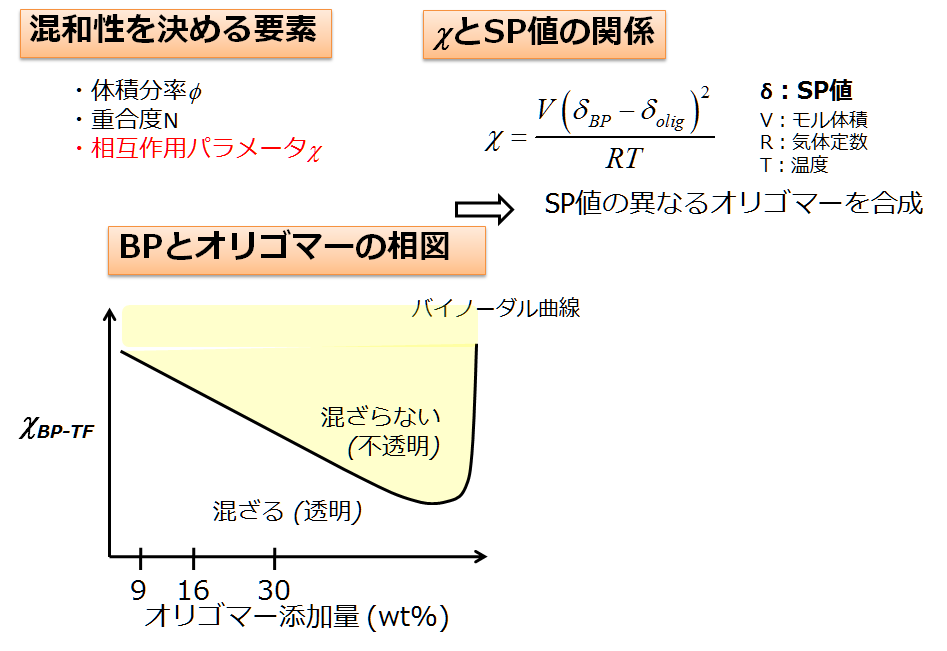
\includegraphics[width=100mm]{souzu_1.png}
		\end{center}
	\end{figure}
\end{frame}

%%%%%
%
\begin{frame}\frametitle{相図による混和性の確認}
	\begin{figure}
		\begin{center}
			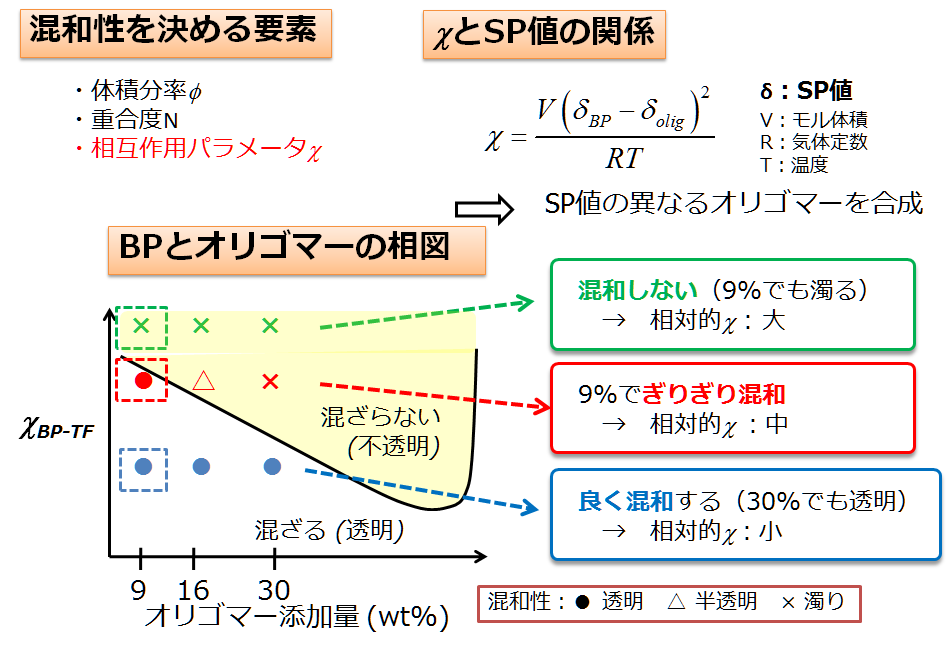
\includegraphics[width=100mm]{souzu_2.png}
		\end{center}
	\end{figure}
\end{frame}

\begin{frame}
	\frametitle{タッキファイヤーの混和性、Tgと耐発泡性}
		\centering
			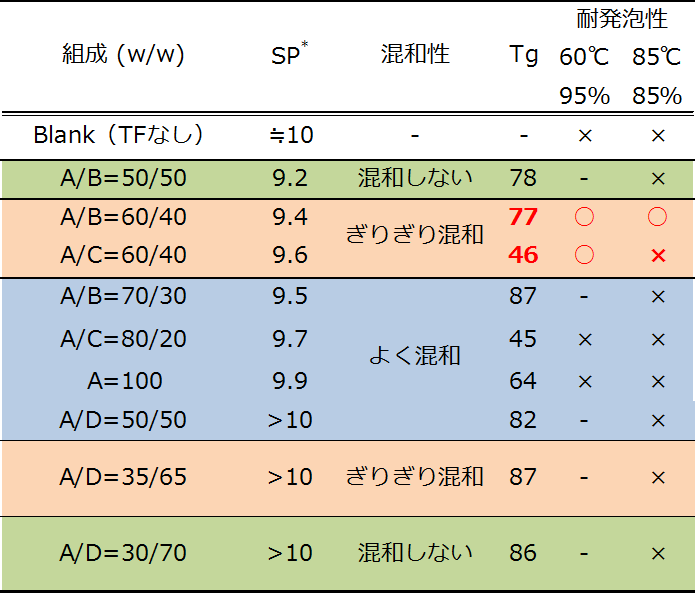
\includegraphics[width=75mm]{TF_table.png}
\end{frame}

\begin{frame}\frametitle{粘着力の測定条件}
	\begin{figure}
		\begin{center}
			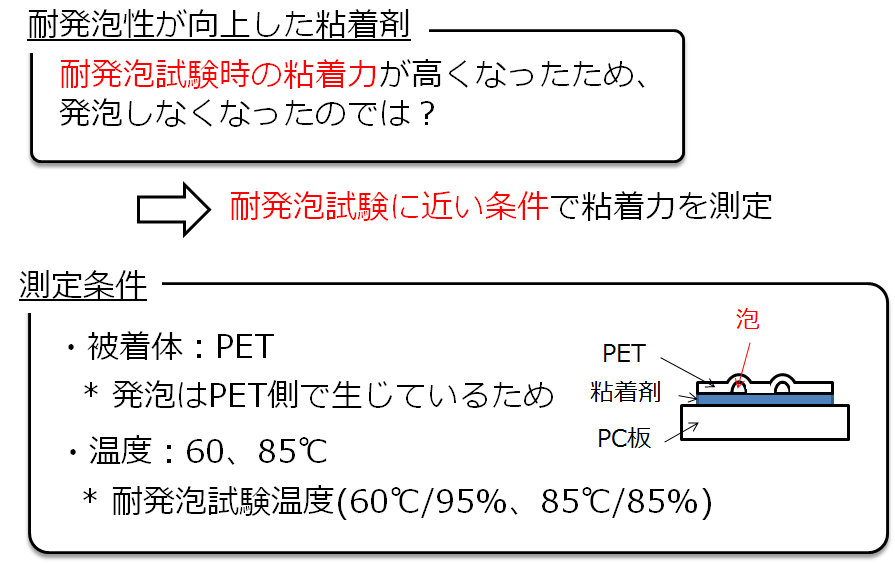
\includegraphics[width=100mm]{adh_1.png}
		\end{center}
	\end{figure}
\end{frame}

%%%%%
%
\begin{frame}\frametitle{耐発泡性と高温での粘着力の関係}
	\begin{figure}
		\begin{center}
			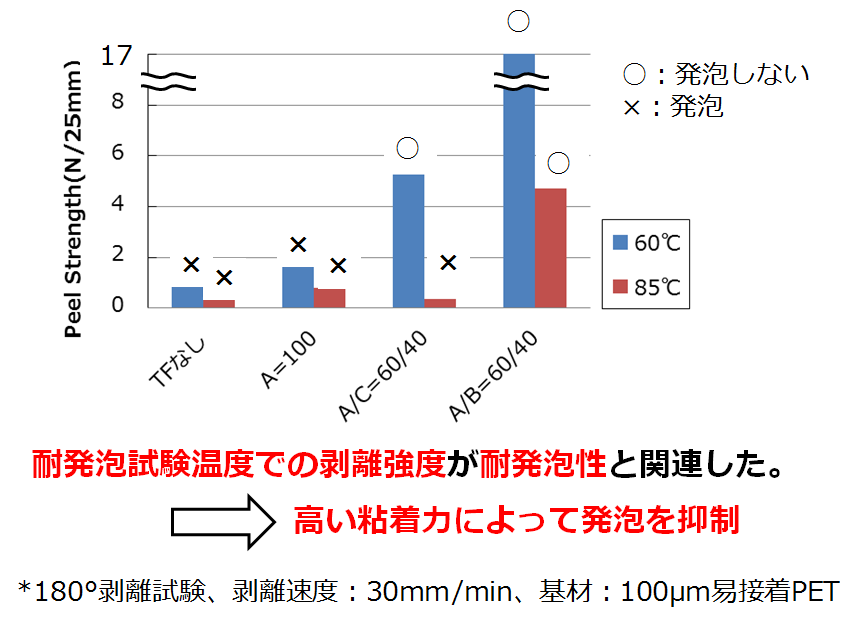
\includegraphics[width=90mm]{adh_2.png}
		\end{center}
	\end{figure}
\end{frame}

\begin{frame}\frametitle{XPS測定条件}
	% 測定:名工大、大型設備基盤センターに依頼
	\begin{columns}[c, onlytextwidth]
		\column{.48\linewidth}
			\begin{block}{X線源条件}
				\begin{itemize}
					\item Al-Kα (1486.6eV)
					\item スポット径=φ100μm
					\item X線入射角=0°
					% (試料測定面の法線に対する角度)
					\item 光電子検出角=45° \\⇒ 約5nmまで観察
				\end{itemize}
			\end{block}
		\column{.48\linewidth}
			\centering
			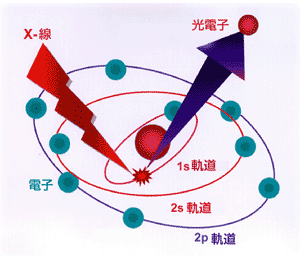
\includegraphics[width=.7\textwidth]{XPS_Genri_1.png}
			\vspace{3mm}
			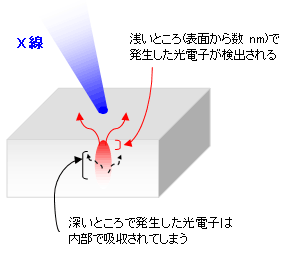
\includegraphics[width=.7\textwidth]{XPS_Genri_3.png}
	\end{columns}
\end{frame}
	
	%%%%%
	%
\begin{frame}\frametitle{ブチルアクリレートの場合}

\begin{figure}
	\begin{center}
		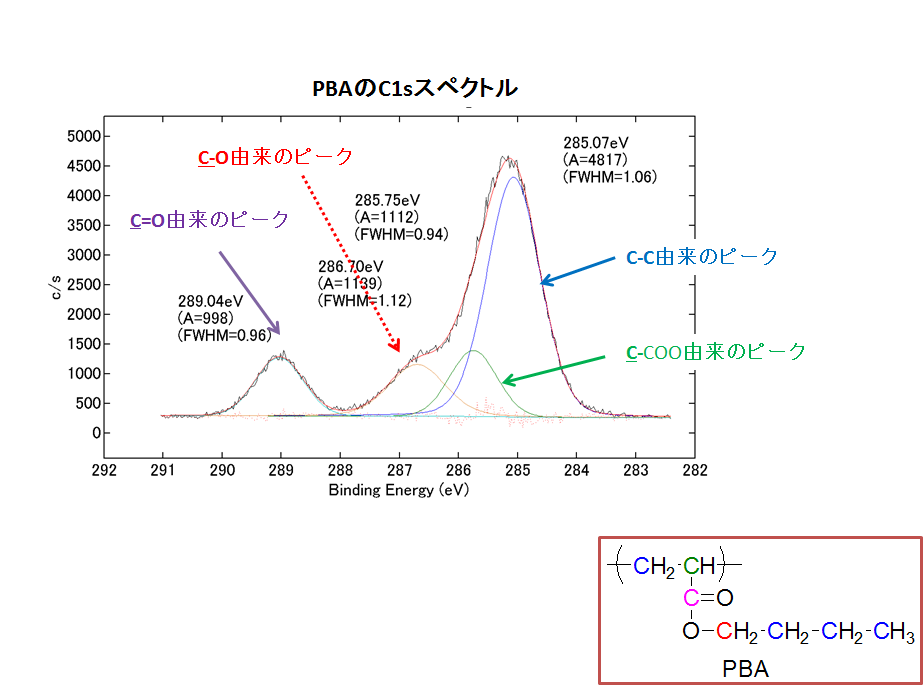
\includegraphics[width=90mm]{XPS_BA.png}
	\end{center}

\end{figure}

\end{frame}

%%%%%
\begin{frame}\frametitle{XPSによるタッキファイヤーの表面偏析}

\vspace{-0.2\baselineskip}
\begin{alertblock}{タッキファイヤーの表面濃度}
約 $9\%$ の添加にもかかわらず、表面はほとんどタッキファイヤーで覆われていた。
\end{alertblock}

\vspace{-0.4\baselineskip}
\begin{figure}
	\begin{center}
		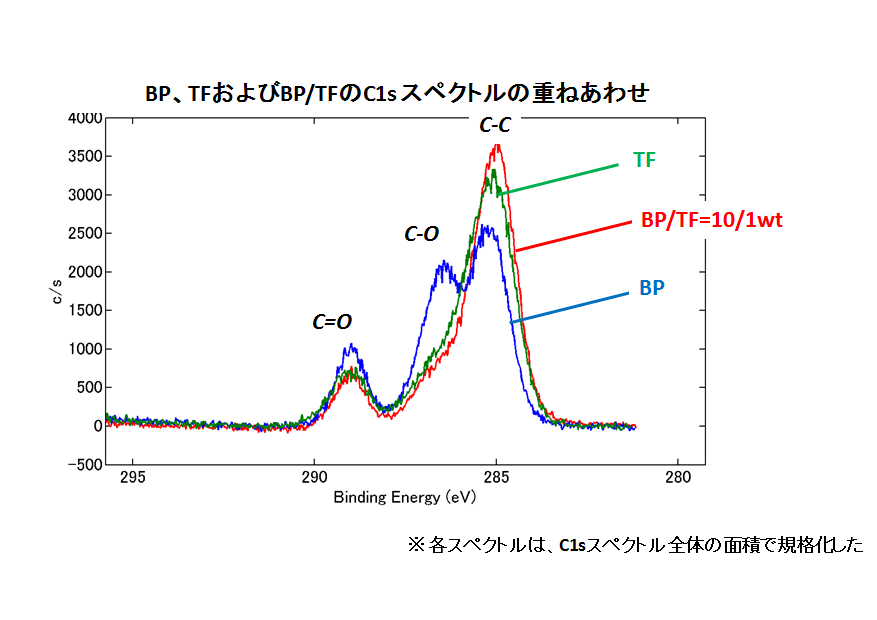
\includegraphics[width=80mm]{XPS_TF.png}
	\end{center}
\end{figure}
\end{frame}
%%%%

\subsection{有効なタッキファイヤーの探索}
\begin{frame}\frametitle{相図による確認}

	\begin{figure}
		\begin{center}
			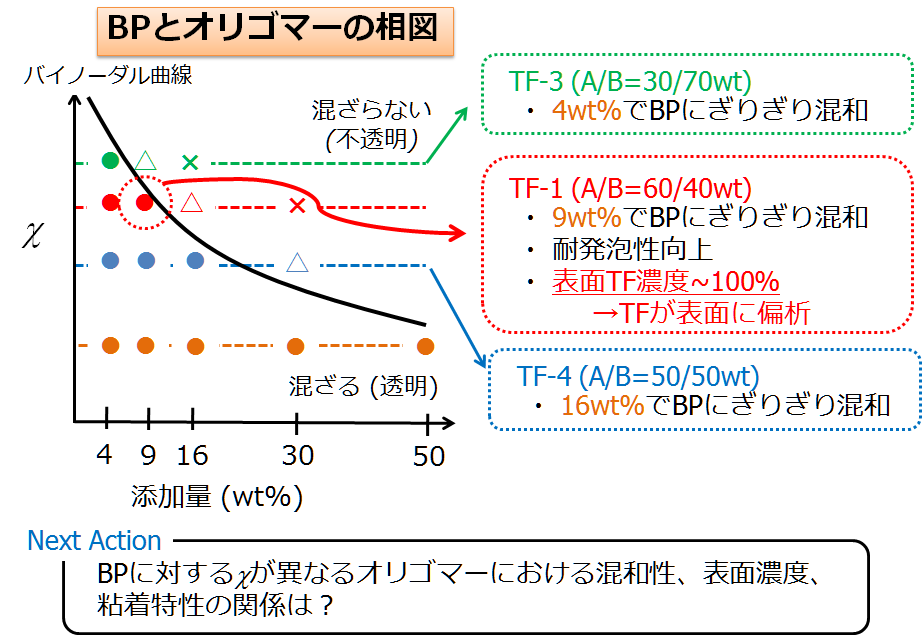
\includegraphics[width=95mm]{tennkaryou_2.png}
		\end{center}
	\end{figure}
	\end{frame}

	
\begin{frame}\frametitle{各種タッキファイヤーの発泡抑制効果}

\large
発泡抑制効果が最大、ピール強度も極大となる添加量で、表面偏析量がほぼ 100\% になっていた。

\begin{columns}
\begin{column}{6 cm}
%{\small 軟 X 線照射で光電子をたたき出す。}
%	\vspace{-10pt}
	\begin{figure}[htbp]
		\begin{center}
			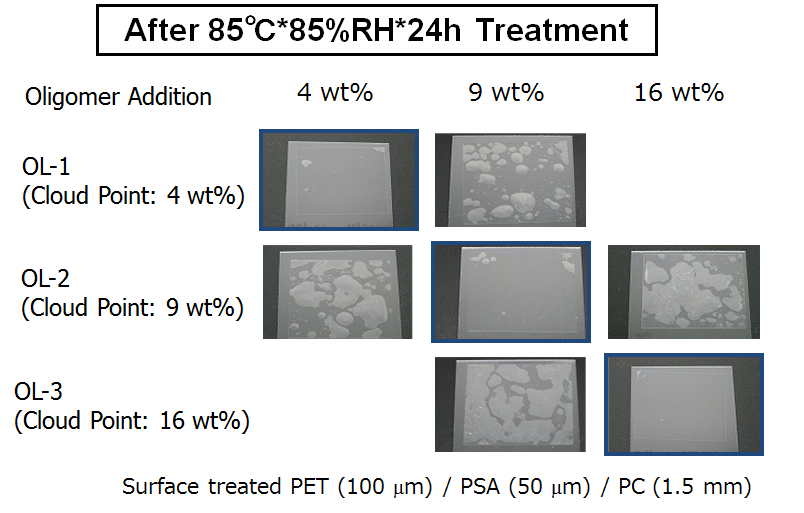
\includegraphics[width=60mm]{tennka_hapou_BW.png}
		\end{center}
	\end{figure}
\end{column}
\begin{column}{6cm}
%	{\small 表面近傍のサンプル中の化学構造に応じたスペクトルを得る。}
%	\vspace{-12pt}
	\begin{figure}[htbp]
		\begin{center}
			\hspace{10pt}
			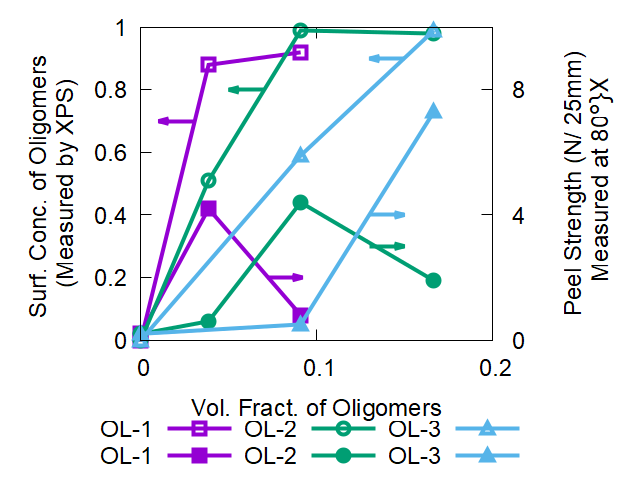
\includegraphics[width=60mm]{Exp_Data_color.png}
		\end{center}
\end{figure}

\end{column}
\end{columns}

\end{frame}

%%%%%%%%%%
\begin{frame}\frametitle{タッキファイヤーの偏析と粘着特性}
	\begin{figure}
		\begin{center}
			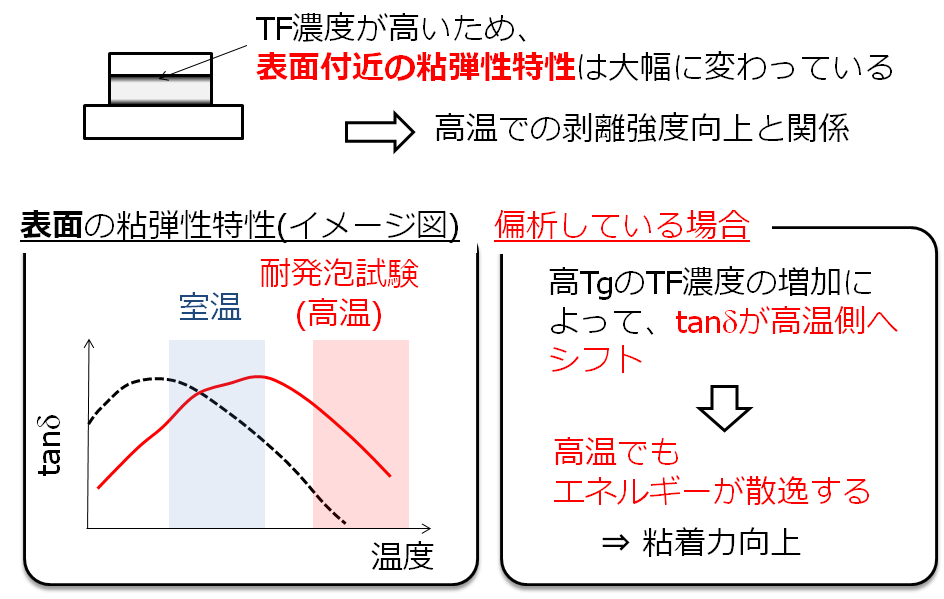
\includegraphics[width=100mm]{PSA2.png}
		\end{center}
	\end{figure}
\end{frame}


\begin{frame}
	\frametitle{「OCA改質用新規タッキファイヤーの開発」のまとめ}
        \begin{boxnote}
            \vspace{-3mm}
            \begin{itemize}
                \item 開発ターゲットの設定
                    \begin{itemize}
                        \item 既存OCAでの発泡を抑制したい
                        \item 界面での粘着力を向上できる材料
                    \end{itemize} 
                \item タッキファイヤーの選択
                    \begin{itemize}
                        \item Tgおよび混和性の異なるタッキファイヤー
                        \item 高Tgで表面偏析が生じるものが有効
                    \end{itemize} 
                \item 有効なタッキファイヤーの探索
                    \begin{itemize}
                        \item 周辺の材料を探索し傾向を確認
                        \item 界面での粘弾性特性を改良していると推定
                    \end{itemize}
            \end{itemize}
        \end{boxnote}
\end{frame}

%%%%%
\section{シミュレーションによる機構の推定}
\subsection{モデル構築のための考え方}
\begin{frame}\frametitle{自由エネルギーによる系の記述}
	\begin{block}{物質の安定な状態 $\Leftrightarrow$ 「自由エネルギーが最小となる状態」} 
		\vspace{-1\baselineskip}
		\begin{align*}
		F &= \color{blue}E\color{black} - \color{green}TS\color{black} \notag \\
			&= \text{\color{blue}内部エネルギー項\color{black}} - \text{\color{green}エントロピー項\color{black}}
		\end{align*}
		%\vspace{-1\baselineskip}
		系の平衡構造を記述可能
	\end{block}
	\begin{itemize}
		\item 実際の実験系\\
			\begin{itemize}
			\item 条件変更で二項がそれぞれ変化$\Leftrightarrow$\color{red}寄与の分割が困難
			\color{black}
			\item 都合の良い効果だけで説明しがち。
		\end{itemize}
		\item シミュレーション(理論的アプローチ)
			\begin{itemize}
			\item これらの効果を\color{red}分割して議論可能\color{black}。
			\item \color{red}筋の通ったモデル構築\color{black}を行える。
			\end{itemize}
	\end{itemize}
\end{frame}
%%%%%
%
\begin{frame}\frametitle{ここでのエントロピーとは}
	\begin{block}{統計力学的エントロピー $S$}
	ボルツマンの関係式により以下のように書くことができる。
	\vspace{-0.5\baselineskip}
	\begin{align*}
	S = k_B \ln W
	\end{align*}
	ここで、$W$は系の取りうる「微視的状態の数」である。
	\end{block}
	\begin{itemize}
	\item FH 格子モデル
		\begin{itemize}
		\item 並進エントロピー\\
		鎖長と無関係に\color{red}重心の配置状態の数のみ\color{black}を数え上げる
		\end{itemize}
	\item 界面の効果を評価するためには
		\begin{itemize}
		\item 形態エントロピー $\Leftarrow$ 高分子の大きさや形を評価\\
		高分子鎖中の\color{red}各セグメントの配置状態\color{black}を数え上げる
		\end{itemize}
	\end{itemize}
\end{frame}
%
\begin{frame}\frametitle{枯渇現象(エントロピー効果)}
	\begin{itemize}
		\item ポリマーが壁(\color{red}基材との界面 or 気体との界面\color{black})に近接
		\begin{itemize}
			\item 壁と重なる部分にセグメントを配置できない
			\item 配置は\color{red}制限を受ける\color{black}
		\end{itemize}
		\item このポリマー鎖の\color{red}形態エントロピーが減少\color{black}する
	%\footnote{重心の位置を固定したという制限の元での、セグメントを配置する場合の数に基づくエントロピー。}
	\end{itemize}

	\begin{figure}[htbp]
		\begin{center}
			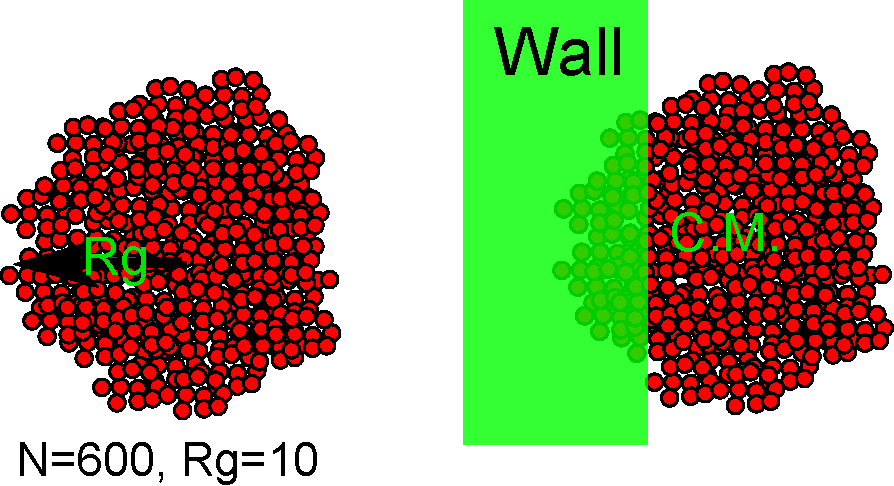
\includegraphics[width=60mm]{polymer_wall.pdf}
		\end{center}
	\end{figure}

\end{frame}

%%%%%
%
\begin{frame}
	\frametitle{ポリマーとオリゴマーの混合物}
	\large
	\begin{itemize}
		\item 壁近傍での形態エントロピー
		\begin{itemize}
	%\large
			\item 慣性半径の大きい高分子量ポリマー\color{red}だけ\color{black}が壁の影響
			\item セグメント数の少ないオリゴマーの形態エントロピーは影響を受けない
		\end{itemize}
		\item 壁近傍での振る舞い
		\begin{itemize}
	%\large
			\item \color{red}オリゴマーを自由に配置\color{black}でき並進エントロピーを獲得
			\item \color{red}ポリマーが枯渇 $\Leftrightarrow$ オリゴマーが偏析\color{black}
		\end{itemize}
	\end{itemize}
	\begin{block}{オリゴマーの偏析}
	相互作用パラメタの影響を考慮することなく、\color{red}「エントロピー効果のみで記述」\color{black}できる。
	\end{block}
\end{frame}

\begin{frame}\frametitle{モデル構築の考え方}
	SUSHI(SCF 計算を利用)によりシミュレーションを行い、エントロピー項と内部エネルギー項とを分割してモデルを構築
	\begin{block}{エントロピー効果の理解}
	セグメント間相互作用パラメタ($\chi$:内部エネルギーに対応)を $\chi = 0$ として、セグメント数の異なるポリマーとオリゴマー混合物の壁近傍での振る舞いを検討。
	\end{block}
	
	\begin{exampleblock}{相図を用いた実験との整合}
	実験と対応できるセグメント間相互作用パラメタを相図から見積もり、内部エネルギーの効果を検討。
	\end{exampleblock}
\end{frame}

\begin{frame}
	\frametitle{「モデル構築の考え方」のまとめ}
        \begin{boxnote}
            \vspace{-3mm}
            \begin{itemize}
                \item 自由エネルギーについて
                    \begin{itemize}
						\item 実験系では寄与の分割が困難
						\item シミュレーションにより筋の通った説明
					\end{itemize} 
                \item エントロピーについて
                    \begin{itemize}
                        \item 並進エントロピーと形態エントロピー変化
                        \item 枯渇現象がこの表面偏析の原因と推定
                    \end{itemize} 
                \item モデル構築の考え方
                    \begin{itemize}
                        \item SUSHI での SCF 計算で形態エントロピーも\\考慮して系全体の平衡構造をシミュレート
                    \end{itemize}
            \end{itemize}
        \end{boxnote}
\end{frame}

\subsection{SUSHIによるシミュレーション}
\begin{frame}
	\frametitle{シミュレーション手法:}
	SUSHIでのSCF(Self Consistent Field)計算
		\begin{columns}
			\begin{column}{6.0cm}
				{\scriptsize
				\begin{block}{無矛盾になるまでループ計算}
				\begin{itemize}
					\item 経路積分:ポテンシャル場の元でポリマー鎖の配置(形態を考慮)を決定
					\item セグメント濃度:ポリマー鎖の配置から算出
					\item 自己無撞着場:セグメント濃度で決まるポテンシャル場
				\end{itemize}
				\end{block}
				}
			\end{column}
			\begin{column}{6.0cm}
				\begin{figure}[!b]
					\begin{center}
						\includegraphics[width=60mm]{scf.png}
					\end{center}
				\end{figure}
			\end{column}
		\end{columns}

		\begin{center}
			{\Large $\Downarrow$}
		\end{center}

		\begin{itemize}
			\item \color{red}形態エントロピーも考慮\color{black}して、自由エネルギーを決定
			\item 系全体の\color{red}平衡構造\color{black}をシミュレート
		\end{itemize}
\end{frame}
%%%%%
%
\begin{frame}\frametitle {オリゴマーとポリマーを等量混合($\chi = 0.0$)}

\begin{itemize}
	\item 鎖長 6 のオリゴマーとポリマー(鎖長: 600)を等量混合
	\item 鎖長の短いオリゴマー成分が、壁近傍に偏析
\end{itemize}

\vspace{-0.5\baselineskip}
\begin{figure}[htbp]
	\begin{center}
		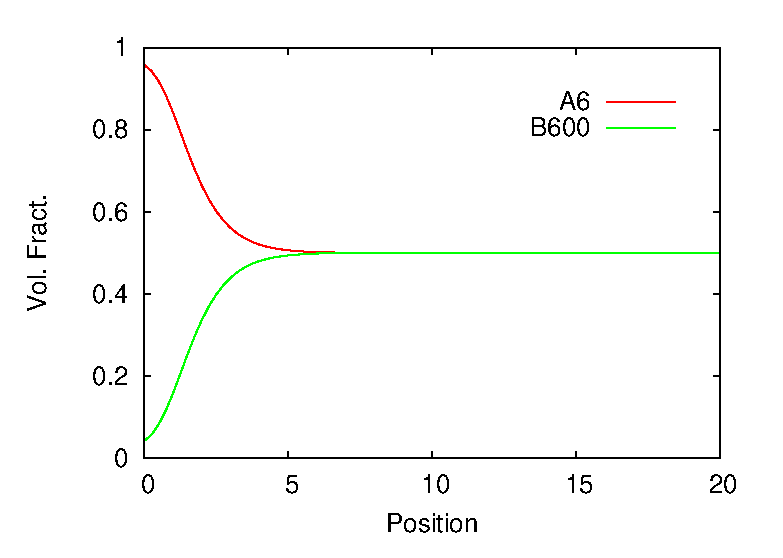
\includegraphics[width=75mm]{Sym_A6B600_Chi_0.eps}
	\end{center}
\end{figure}

\begin{center}
\vspace{-0.5\baselineskip}
{\small A6 と B600 を $\phi_A = \phi_B = 0.5$ とした場合の偏析}
\end{center}

\end{frame}

%%%%%
%
\begin{frame}\frametitle{等量混合での鎖長の効果($\chi = 0.0$)}

\begin{itemize}
	\item オリゴマー鎖長が長くなると、偏析領域および量が増加
	\item ポリマーの慣性半径(10程度)まで偏析
\end{itemize}

\vspace{-0.5\baselineskip}
\begin{figure}[htbp]
	\begin{center}
		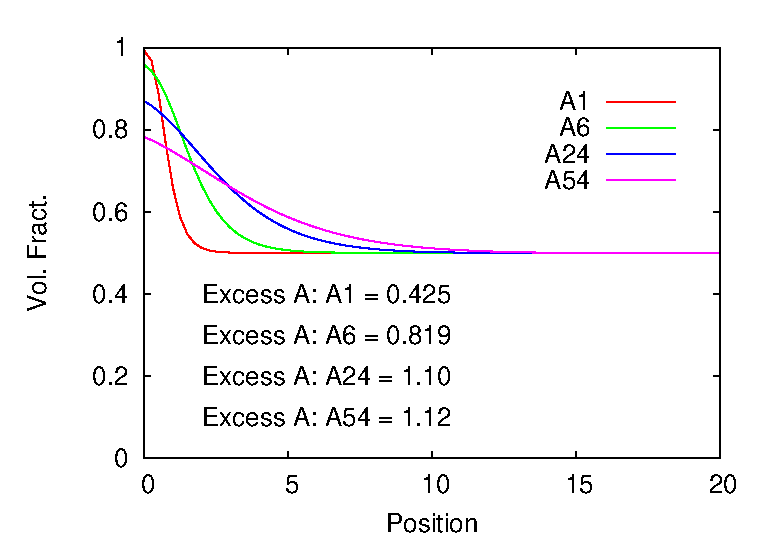
\includegraphics[width=75mm]{Sym_B600_All.eps}
	\end{center}
\end{figure}

\begin{center}
\vspace{-0.5\baselineskip}
{\small B600 を異なる鎖長のオリゴマーと等量混合した偏析}
\end{center}

\end{frame}

%%%%%
\begin{frame}\frametitle{$N_A = 6$と$N_B = 600$混合物の相図}
	\begin{itemize}
		\item ポリマーとオリゴマーの混合物
		\begin{itemize}
			\item バイノーダル線が非対称
		\end{itemize}
		\item 相分離後
		\begin{itemize}
			\item ほぼオリゴマーのみの相(相図の右側)
			\item 少量のオリゴマーとポリマーが混合した相(相図の左側)
		\end{itemize}
	\end{itemize}

	\vspace{-0.5\baselineskip}
	\begin{figure}[htbp]
		\begin{center}
			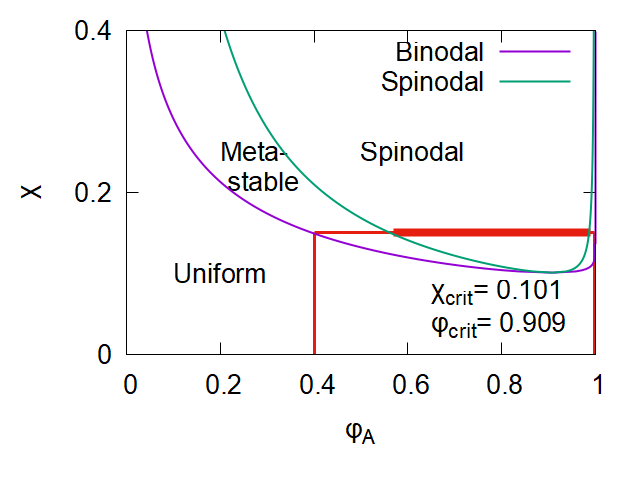
\includegraphics[width=65mm]{PD_6_600_4.png}
		\end{center}
	\end{figure}
\end{frame}

%%%%%
%
\begin{frame}
	\frametitle{壁存在下のシミュレーション}
	\begin{itemize}
		\item 実験系
		\begin{itemize}
		\item 熱揺らぎの影響大$\Leftrightarrow$バイノーダル点で相分離
		\end{itemize}
		\item 壁存在下のシミュレーション
		\begin{itemize}
			\item 壁のない条件(たとえば、周期境界条件)
			\begin{itemize}
				\item スピノーダル領域で相分離が発生
				\item 準安定領域では一様混合
			\end{itemize}
			\item バイノーダル線の内側(Metastable 領域)
			\begin{itemize}
				\item システム内のほぼすべてがオリゴマーで充足
				\item 壁近傍で、局所的な相分離
			\end{itemize}
		\end{itemize}
	\end{itemize}

	\begin{alertblock}{シミュレーションの考え方}
	相図に基づいて実験と対比できる $\chi$ パラメタを設定し、\\
	偏析をシミュレーション
	\end{alertblock}
\end{frame}

%%%%%
\begin{frame}\frametitle{相互作用パラメタ $\chi$ の実験との対比}

\begin{alertblock}{シミュレーションの考え方}
相図に基づいて実験と対比できる $\chi$ パラメタを設定し、\\
偏析をシミュレーション
\end{alertblock}

\begin{columns}
	\begin{column}{6.0cm}
%		\begin{itemize}
%			\item 「混合の自由エネルギー変化」
%			\begin{itemize}
%				\item 一様状態?$\Leftrightarrow$相分離?
%			\end{itemize}
%			\item 自由エネルギー曲線の例
%			\begin{itemize}
%				\item 極小値一つ $\Rightarrow$ 一様混合
%				\item 極小値が二つ $\Rightarrow$ 相分離
%			\end{itemize}
%		\end{itemize}
		\vspace{-0.5\baselineskip}
		\begin{figure}[htbp]
			\begin{center}
				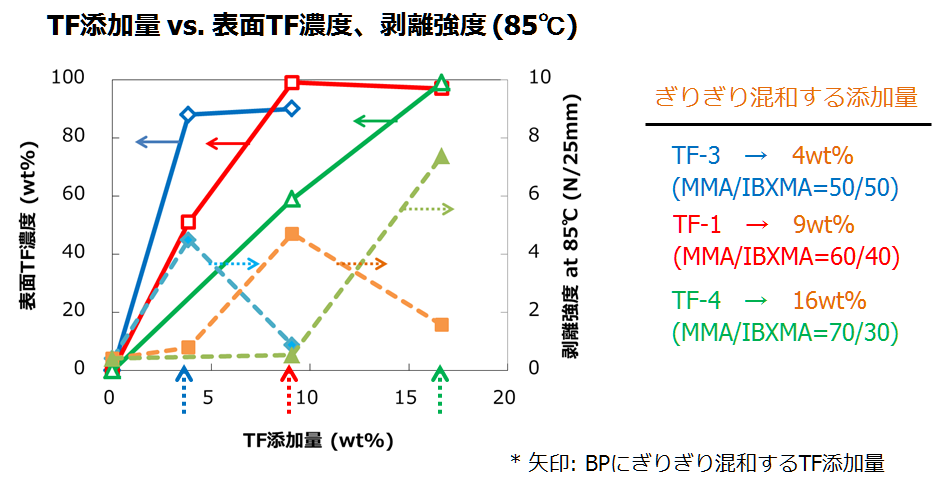
\includegraphics[width=60mm]{nakamura-2.png}
			\end{center}
		\end{figure}
		\begin{center}
			\vspace{-0.5\baselineskip}
			{\footnotesize 実験でのイメージ図}
		\end{center}
	\end{column}
	\begin{column}{6.0cm}
%		\begin{block}{相図}
%		{\footnotesize $\chi$パラメタを縦軸に系の振る舞いを記述する図}
%		\end{block}
		\vspace{-1\baselineskip}
		\begin{figure}[htbp]
			\begin{center}
				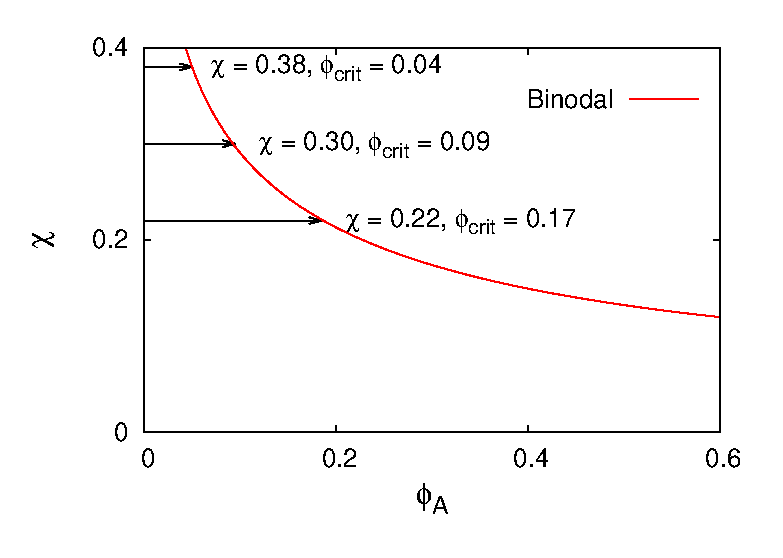
\includegraphics[width=60mm]{PD_6_600_3.eps}
			\end{center}
		\end{figure}
		\begin{center}
			\vspace{-1\baselineskip}
			{\footnotesize 理論的相図と実験の対比}
		\end{center}
	\end{column}
\end{columns}

\end{frame}

%%%%%
\begin{frame}\frametitle{$\chi_{AB} = 0.3$ :TF-1($9\%$ まで一様混合)を模擬}

\begin{itemize}
	\item オリゴマー量の増加$\Leftrightarrow$界面でのオリゴマー偏析量が増加
	\item 析出厚みも暫時増加
	\item Metastabel 領域($\phi_A = 0.1$)で局所的な相分離
\end{itemize}

\vspace{-0.5\baselineskip}
\begin{figure}[htbp]
	\begin{center}
		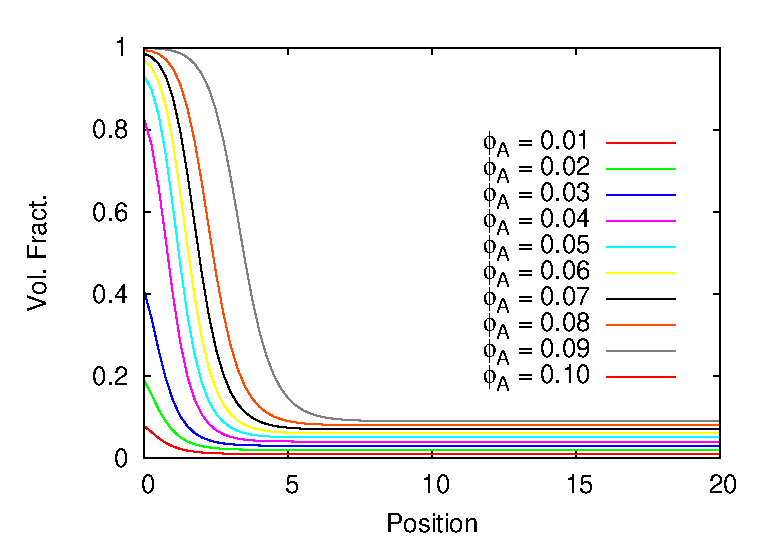
\includegraphics[width=75mm]{A6_B600_Chi_03_chiS_0.0_all.eps}
	\end{center}
\end{figure}
\end{frame}

\begin{frame}
	\frametitle{「SUSHIによるシミュレーション」のまとめ}
        \begin{boxnote}
            \vspace{-3mm}
            \begin{itemize}
                \item シミュレーション手法
                    \begin{itemize}
						\item SUSHIによるSCF計算
						\item 系全体の平衡構造をシミュレート
                        \item 形態エントロピー効果だけで枯渇現象
                    \end{itemize} 
                \item 相互作用パラメタχの実験との対比
                    \begin{itemize}
                        \item 相図に基づいて実験と対比できる χ パラメタ
                        \item 表面偏析に対応するシミュレーション
                    \end{itemize} 
                % \item 実験結果との整合性の検討
                %     \begin{itemize}
                %         \item 表面偏析に関する実験結果との整合性を確認
                %         \item 接着性の発現機構に対するイメージを深化
                %     \end{itemize}
            \end{itemize}
        \end{boxnote}
\end{frame}
%%%%%
\subsection{実験結果との整合性の検討}
\begin{frame}\frametitle{XPSの角度依存性}

{\small %光電子は、他の原子核に衝突することで非弾性散乱する。

平均自由工程($\lambda$):光電子密度が$\exp \left(-\dfrac{d}{\lambda}\right) = \dfrac{1}{e}$ になる距離

有機物中では $\lambda \simeq$ 3 nm}
\begin{columns}
\begin{column}{4cm}
	\vspace{-10pt}
	\begin{figure}[htbp]
		\begin{center}
			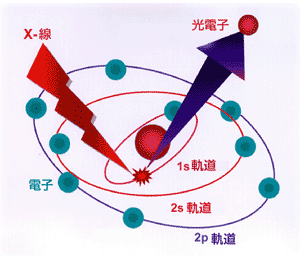
\includegraphics[width=25mm]{XPS_Genri_1.png}
		\end{center}
	\end{figure}
	\vspace{-20pt}
	\begin{figure}[htbp]
		\begin{center}
			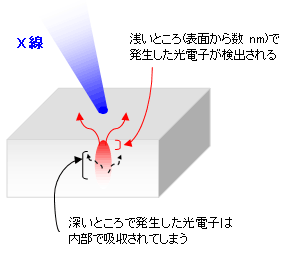
\includegraphics[width=30mm]{XPS_Genri_3.png}
		\end{center}
	\end{figure}
\end{column}
\begin{column}{7cm}
	\begin{figure}[htbp]
		\begin{center}
			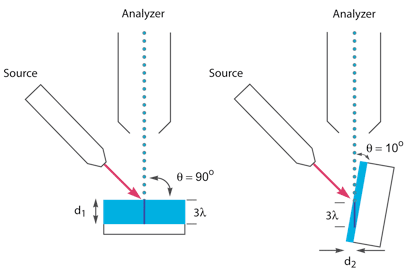
\includegraphics[width=55mm]{XPS_KAKUDO.png}
		\end{center}
\end{figure}

\vspace{-5pt}
{\small 角度依存性:$\exp \left(-\dfrac{d}{\lambda \sin \theta}\right)$}

\end{column}
\end{columns}

\end{frame}

%%%%%
\begin{frame}\frametitle{XPS(X-ray Photo-electron Spectroscopy) 測定}

\begin{itemize}
	\item XPS測定
	\begin{itemize}
	\item XPS:X 線照射により放出される電子(光電子)を検出
	\item 試料内部からの電子は、試料表面からの距離 \color{red}$l_{f} d$\color{black} と平均自由行程(\color{red}$\lambda \sin \theta$\color{black})との比にしたがって\color{red}指数関数的に減衰\color{black}。
	\end{itemize}
%	\item 測定シグナル($\phi^{XPS} (sim)$)
%	\begin{itemize}
%	\item を、フィッティングパラメタ $l_f$ を用いた以下の表式により対応。
%%
%	\end{itemize}
\end{itemize}
%\vspace{-0.1\baselineskip}
\begin{equation*}
\begin{cases}
	\phi_A^{{XPS}_(sim)} = 
		\dfrac{\sum_{d} \phi_A(d) \cdot \exp \left(- \color{red}l_{f}\color{black}d/\lambda \sin \theta \right) } 
		{\sum_{d} \exp \left(- \color{red}l_{f}\color{black}d/\lambda \sin \theta \right)} \\[8pt]
	\phi_B^{{XPS}_(sim)} = 
		\dfrac{\sum_{d} \phi_B(d) \cdot \exp \left(- \color{red}l_{f}\color{black}d/\lambda \sin \theta \right) } 
		{\sum_{d} \exp \left(- \color{red}l_{f}\color{black}d/\lambda \sin \theta \right)}
\end{cases}
\end{equation*}

%\vspace{-0.5\baselineskip}
%\begin{equation*}
%	\begin{cases}
%		\phi_A^{XPS} (sim) = \dfrac{\sum_d \phi_A(d) \cdot \exp(-\lambda d \sin \theta)}{\sum_d \exp(- \lambda d \sin \theta) } \\[12pt]
%		\phi_B^{XPS} (sim) = \dfrac{\sum_d \phi_B(d) \cdot \exp(-\lambda d \sin \theta)}{\sum_d \exp(- \lambda d \sin \theta) }
%	\end{cases}
%\end{equation*}

%\vspace{-0.5\baselineskip}
\begin{block}{}
\color{red}$l_f$\color{black}をフィッティングパラメタとして、実験での \color{red}$\phi_A^{XPS}$\color{black} と\\
シミュレーションの偏析プロファイル\color{red} $\phi(d)$ を対応\color{black}させ、\\
シミュレーション長さ\color{red} $d$ と実験長さの関係\color{black}を明らかに。
\end{block}
\end{frame}


%%%%%
\begin{frame}\frametitle{XPS測定:フィッティングの評価}

\begin{itemize}
	\item $\chi_{AB} = 0.3$で各オリゴマー量での$\phi_A^{{XPS}_(sim)}$
	\begin{itemize}
		\item 実験での測定値:$\phi_A = 0.04 \leftrightarrow \phi_A^{XPS} = 0.5 $(黒点線)
		\item $l_f \simeq 4.0$ 程度が妥当
	\end{itemize}
\end{itemize}

\vspace{-0.5\baselineskip}
\begin{figure}[htbp]
	\begin{center}
		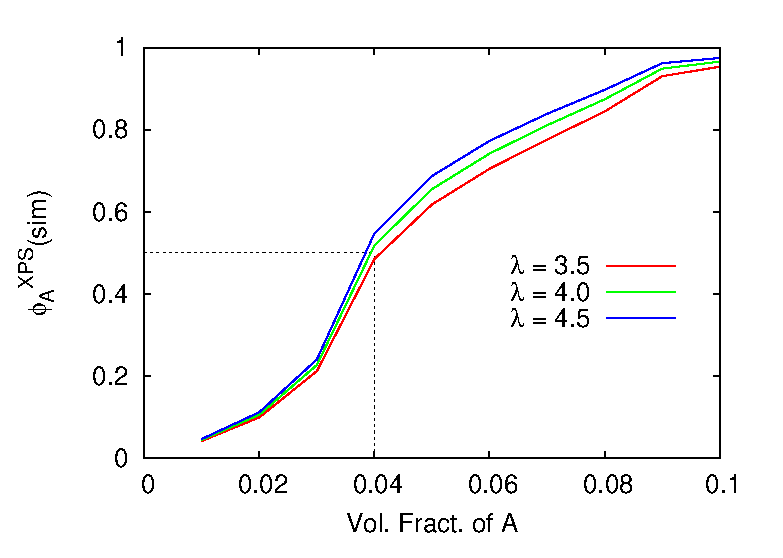
\includegraphics[width=75mm]{XPS_Chi_sin_03.eps}
	\end{center}
\end{figure}

%\begin{center}
%\vspace{-0.5\baselineskip}
%{\small A6 と B600のブレンド、$\chi_{AB} = 0.3$}
%\end{center}

\end{frame}

%%%%%
\begin{frame}\frametitle{XPS測定:$l_f = 4.0$ での実験との比較}

\begin{columns}
	\begin{column}{6.0cm}
%		\begin{block}{相図}
%		{\footnotesize $\chi$パラメタを縦軸に系の振る舞いを記述する図}
%		\end{block}
		\vspace{-1\baselineskip}
		\begin{figure}[htbp]
			\begin{center}
				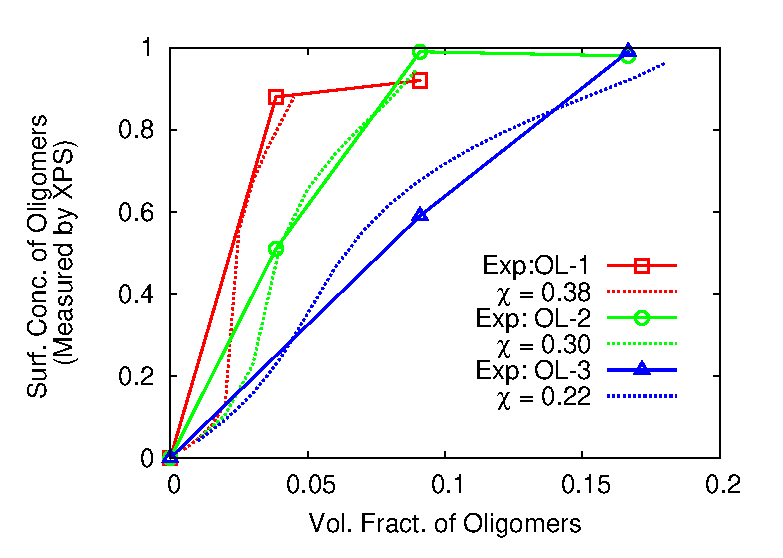
\includegraphics[width=60mm]{XPS_Lf_4_sin_45.eps}
			\end{center}
		\end{figure}
%		\begin{center}
%			\vspace{-1\baselineskip}
%			{\footnotesize $\lambda = 0.9$ での実験結果との比較}
%		\end{center}
	\end{column}
	\begin{column}{6.0cm}
%		\begin{itemize}
%			\item 「混合の自由エネルギー変化」
%			\begin{itemize}
%				\item 一様状態?$\Leftrightarrow$相分離?
%			\end{itemize}
%			\item 自由エネルギー曲線の例
%			\begin{itemize}
%				\item 極小値一つ $\Rightarrow$ 一様混合
%				\item 極小値が二つ $\Rightarrow$ 相分離
%			\end{itemize}
%		\end{itemize}
		\vspace{-0.5\baselineskip}
		\begin{figure}[htbp]
			\begin{center}
				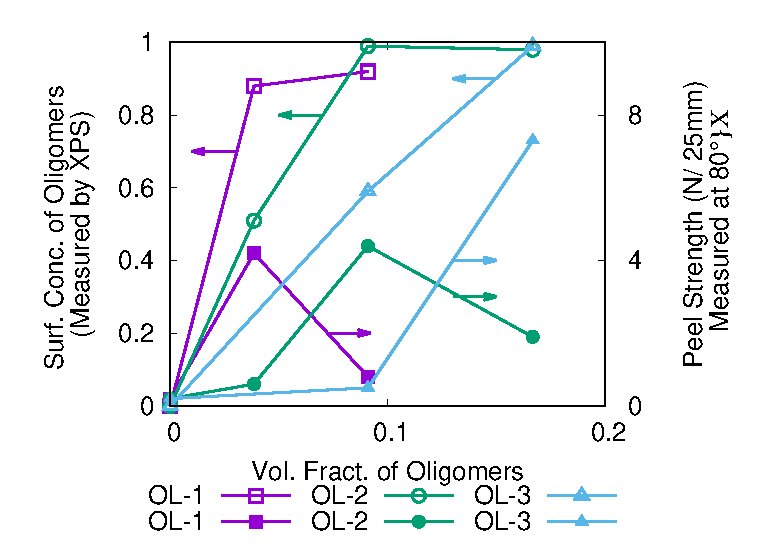
\includegraphics[width=60mm]{Exp_Data_color.eps}
			\end{center}
		\end{figure}
%		\begin{center}
%			\vspace{-0.5\baselineskip}
%			{\footnotesize 実験でのイメージ図}
%		\end{center}
	\end{column}
\end{columns}

\begin{alertblock}{$l_f = 4.0$ でのシミュレーション}
相図に基づいた $\chi$ パラメタ($\chi = 0.22, 0.30, 0.38$)から\\シミュレートした$\phi_A^{XPS}$ が実験結果と非常に良い一致
\end{alertblock}
\end{frame}


%%%%%
\begin{frame}\frametitle{D-SIMSとの整合性}
D-SIMS(Secondary Ion Mass Spectrometry) の測定結果との整合性を確認した。
	\begin{columns}
		\begin{column}{6cm}
				\centering
				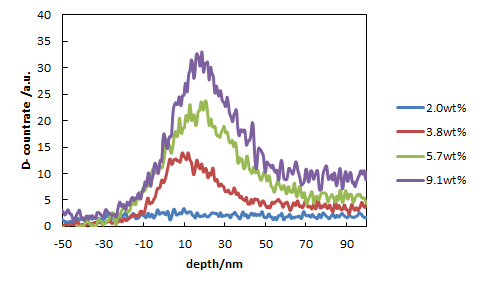
\includegraphics[width=.8\textwidth]{D_SIMS_exp.png}

					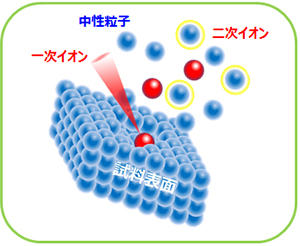
\includegraphics[width=.6\textwidth]{SIMS.jpg}
			
			% \begin{figure}[htbp]
			% 	\begin{center}
					
			% 	\end{center}
			% 	\caption{D-SIMS 測定結果}
			% \end{figure}
		\end{column}
		\begin{column}{5cm}
			\begin{figure}[htbp]
				\begin{center}
					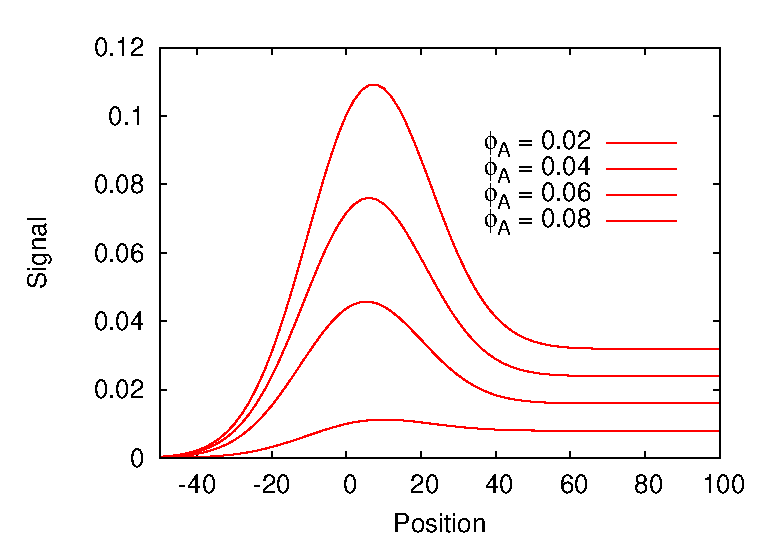
\includegraphics[width=50mm]{Chi_03_Lf_4.0_SIMS_4.eps}
				\end{center}
				\caption{SUSHI で得たプロファイルからの計算}
		\end{figure}
		\end{column}
	\end{columns}
\end{frame}
% %%%%%
% % \subsection{接着強度の改善機構の推定}


%%%%%
\begin{frame}\frametitle{偏析条件下での$T_g$}

\begin{itemize}
	\item Fox の式により、体積分率から局所的な$T_g$を算出
	\begin{itemize}
	\item オリゴマー量の増加$\Rightarrow$界面近傍での高$T_g$領域が厚化
	\item バイノーダル線以上($\phi_A = 0.1$)$\Rightarrow$局所的な相分離
	\end{itemize}
\end{itemize}

\begin{columns}
	\begin{column}{6.0cm}
		\vspace{-1\baselineskip}
		\begin{figure}[htbp]
			\begin{center}
				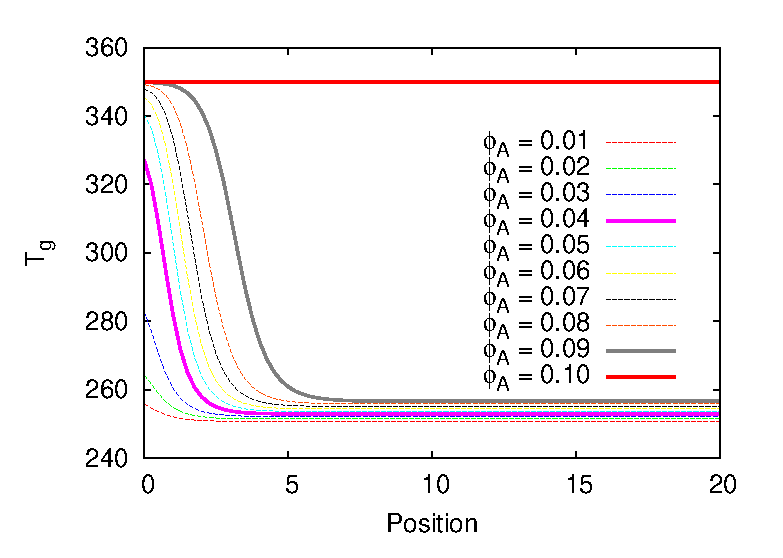
\includegraphics[width=60mm]{A6_B600_Chi_03_chiS_0.0_Tg.eps}
			\end{center}
		\end{figure}
		\begin{center}
			\vspace{-0.5\baselineskip}
			{\footnotesize 偏析条件下での$T_g$($\chi = 0.3$)}
		\end{center}
	\end{column}
	\begin{column}{6.0cm}
%		\pause
		\begin{block}{}
		\vspace{-0.5\baselineskip}
		{\footnotesize 
		\begin{itemize}
		\item 高$T_g$領域が厚化$\Rightarrow$剥離強度上昇
		\item 局所的な相分離$\Rightarrow$剥離強度の低下
			\end{itemize}
		}
		\end{block}
		\vspace{-1\baselineskip}
		\begin{figure}[htbp]
			\begin{center}
				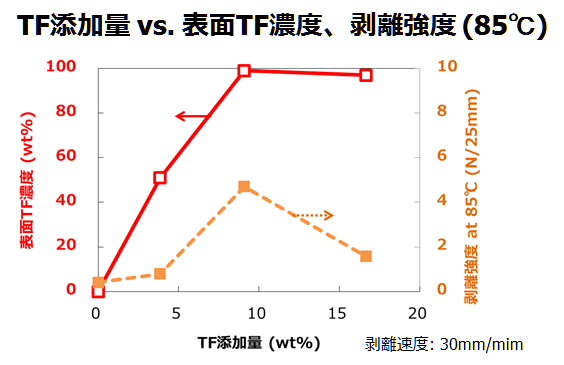
\includegraphics[width=60mm]{nakamura-1.png}
			\end{center}
		\end{figure}
%		\begin{center}
%			\vspace{-1\baselineskip}
%			{\footnotesize 実験結果}
%		\end{center}
	\end{column}
\end{columns}

\end{frame}


%%%%%
\begin{frame}\frametitle{実験に対応した$T_g$プロファイル}

% \vspace{-0.5\baselineskip}
\begin{itemize}
	\item $\chi_{AB}: 0.38 \rightarrow 0.30$ :主として厚みが変化
	\item $\chi_{AB}: 0.30 \rightarrow 0.22$ :プロファイルが滑らかに
\end{itemize}

\vspace{-3mm}

\begin{columns}
	\begin{column}{.48\textwidth}
		\centering
				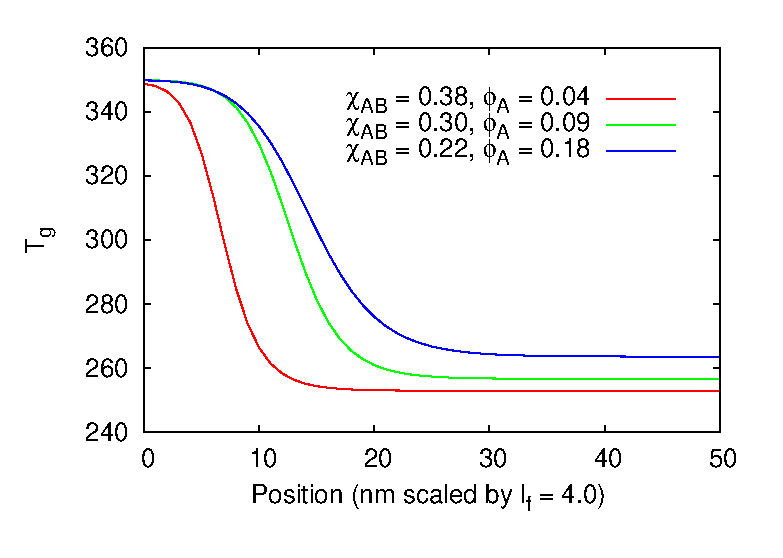
\includegraphics[width=60mm]{Tg.eps}

			\vspace{-3mm}
			{\footnotesize 実験に対応した$T_g$($\chi_{AB} = 0.22, 0.3, 0.38$)}
	\end{column}
	\begin{column}{.48\textwidth}

		% \vspace{-1\baselineskip}
		\begin{figure}[htbp]
			\begin{center}
				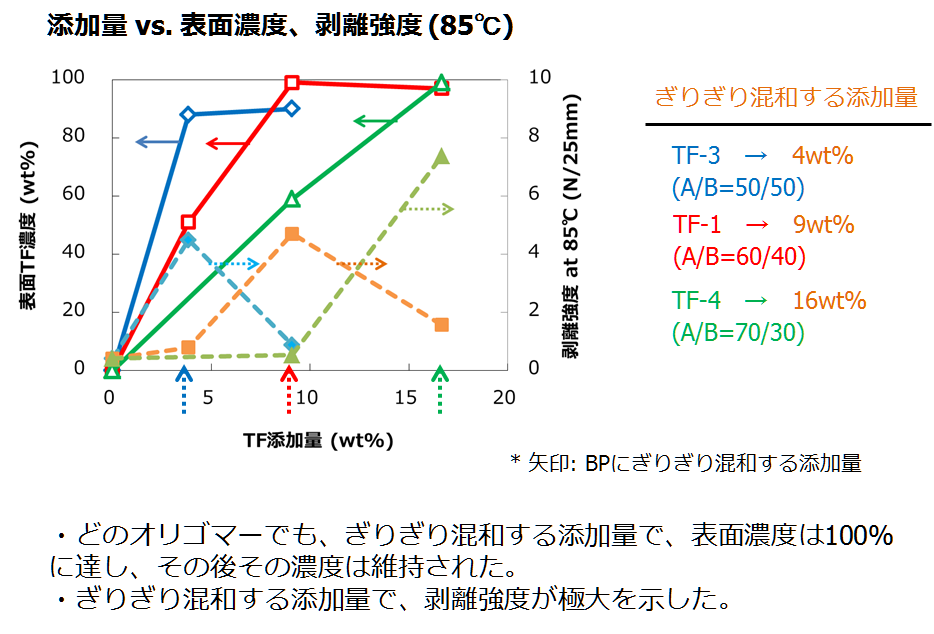
\includegraphics[width=.85\textwidth]{tennkaryou_3.png}
			\end{center}
		\end{figure}
		
		\vspace{-5mm}
		% \vspace{-1.8\baselineskip}
		\begin{figure}[htbp]
			\begin{center}
				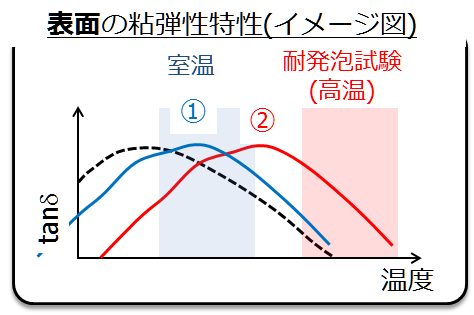
\includegraphics[width=.85\textwidth]{nakamura-3.png}
			\end{center}
		\end{figure}

	\end{column}
\end{columns}

\end{frame}


%%%%%
%\subsection{まとめ}
%
\begin{frame}\frametitle{まとめ}
「ぎりぎりの相溶性のタッキファイヤーが被着体界面に偏析し、接着力が向上する」という実験結果と対応できるモデル構築を目的として、シミュレーションを行った。

\begin{block}{基礎的な事項}
\begin{itemize}
	\item エントロピー効果
	\begin{itemize}
		\item 壁近傍にオリゴマーが偏析
		\item 偏析の厚さは、ポリマーの慣性半径と同程度のオーダー
	\end{itemize}
	\item 内部エネルギー関連
	\begin{itemize}
		\item バイノーダル線の内側(準安定領域)で局所的な相分離
		\item 一様混合領域でバイノーダル線に漸近$\Rightarrow$偏析量が急増
	\end{itemize}
\end{itemize}
\end{block}

\end{frame}

%%%%%
\begin{frame}\frametitle{まとめ}

\begin{center}
\color{red}実験結果との対比\color{black}
\end{center}

\begin{columns}
	\begin{column}{6.0cm}
	\vspace{-1\baselineskip}
	{\scriptsize
		\begin{itemize}
			\item XPS測定とシミュレーションとの整合
		\end{itemize}
	\vspace{-1\baselineskip}
		\begin{figure}[htbp]
			\begin{center}
				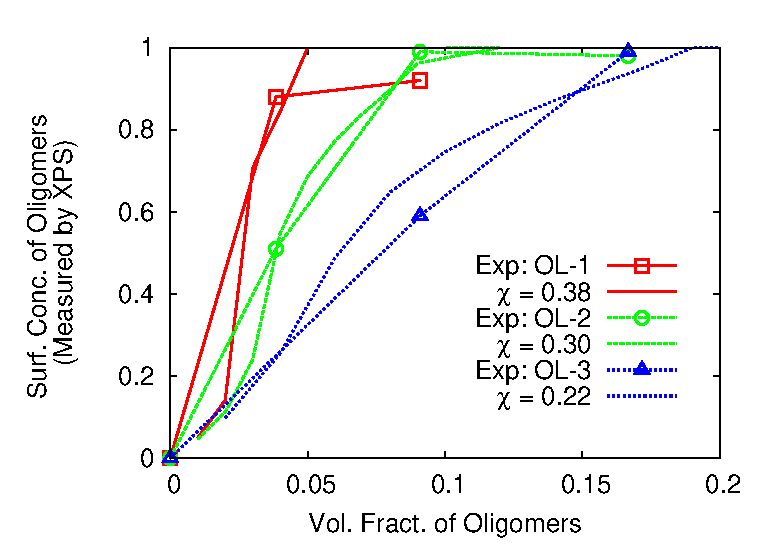
\includegraphics[width=35mm]{XPS_sin_45.eps}
			\end{center}
		\end{figure}

	\vspace{-1\baselineskip}
		\begin{itemize}
			\item 偏析厚み:数 $\sim$ 数 $10 nm$ 程度
		\end{itemize}
		
	\vspace{-1\baselineskip}
		\begin{figure}[htbp]
			\begin{center}
				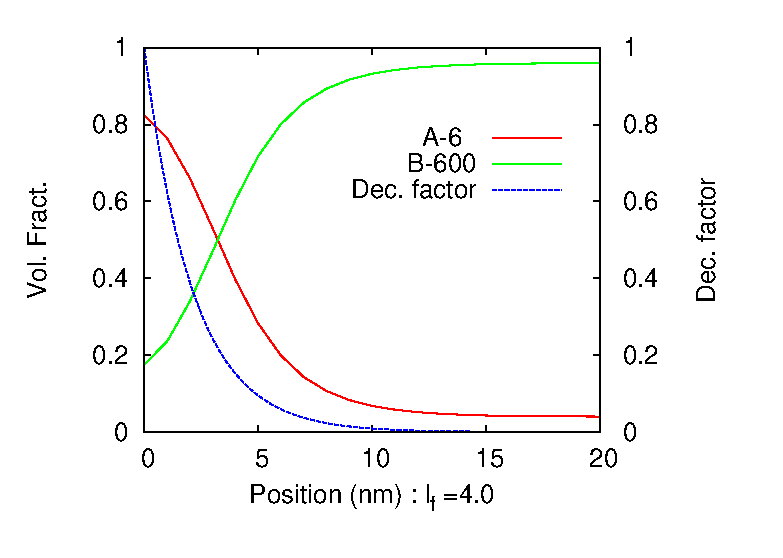
\includegraphics[width=35mm]{A6_B600_Chi_03_chiS_0.0_totalA_0.04.eps}
			\end{center}
		\end{figure}
	}
	\end{column}

	\begin{column}{6.0cm}
	\vspace{-1\baselineskip}
	{\scriptsize
		\begin{itemize}
			\item 相分離ぎりぎり $\Leftrightarrow$ 接着強度が良好
		\end{itemize}
		
		\vspace{-1\baselineskip}
		\begin{figure}[htbp]
			\begin{center}
				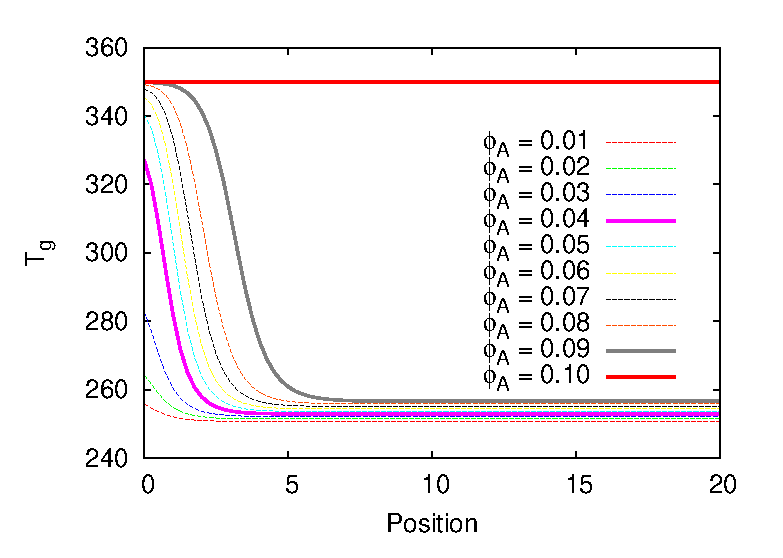
\includegraphics[width=35mm]{A6_B600_Chi_03_chiS_0.0_Tg.eps}
			\end{center}
		\end{figure}

		\vspace{-1\baselineskip}
		\begin{itemize}
			\item 接着強度の向上 $\Leftrightarrow$ 界面プロファイル?
		\end{itemize}
		
		\vspace{-1\baselineskip}
		\begin{figure}[htbp]
			\begin{center}
				\includegraphics[width=35mm]{Tg.eps}
			\end{center}
		\end{figure}
	}
	\end{column}
\end{columns}

\end{frame}

%%%%%
\begin{frame}\frametitle{まとめ}

シミュレーションを用いて、実験結果を説明できる\color{red}モデルを構築\color{black}し、接着性の\color{red}発現機構に対するイメージ\color{black}を得た。

\vspace{-0.5\baselineskip}
\begin{figure}[!b]
	\begin{center}
		\includegraphics[width=80mm]{Exp_Data_color.eps}
	\end{center}
\end{figure}

\end{frame}



\begin{frame}
	\frametitle{「シミュレーションによる機構の推定」の\\まとめ}
        \begin{boxnote}
            \vspace{-3mm}
            \begin{itemize}
                \item モデル構築の考え方
                    \begin{itemize}
						\item 自由エネルギーでの形態エントロピー変化
                        \item 枯渇現象がこの表面偏析の原因と推定
                    \end{itemize} 
                \item SUSHIによるシミュレーション
                    \begin{itemize}
                        \item シミュレーションによる解析を計画
                        \item 基本的な挙動が再現可能
                    \end{itemize} 
                \item 実験結果との整合性の検討
                    \begin{itemize}
                        \item 表面偏析に関する実験結果との整合性を確認
                        \item 接着性の発現機構に対するイメージを深化
                    \end{itemize}
            \end{itemize}
        \end{boxnote}
\end{frame}






%
%%%%%
% \begin{frame}
% %[plain]
% \begin{block}{}
% 	\begin{center}
% 	\LARGE{おしまい}

% 	\large{ご清聴ありがとうございました。}
% 	\end{center}
% \end{block}
% \end{frame}


%%%%%%%
%%%\subsection{SUSHIによるSCF計算}
%%
%\begin{frame}\frametitle{SUSHIの計算条件(エントロピー効果)}
%
%エントロピー効果だけを検討するために、\color{red}相互作用パラメタ $\chi = 0.0$ の無熱状態\color{black}として、シミュレーションを行った。
%\begin{itemize}
%	\item ポリマーとオリゴマー
%        \begin{itemize}
%		\item オリゴマーはAセグメント、高分子量のポリマーはBセグメントから構成されるものとした。
%		\item ポリマーのセグメント数は $N_B = 600$ で固定し、オリゴマーは、それぞれ$N_{\rm{A}} = 1, 6, 24, 54$とした。
%        \end{itemize}
%	\item システム\footnote{壁から十分離れた点における体積分率が一定となるように、システムサイズを設定した。}
%	\begin{itemize}
%		\item 一次元とした。
%		\item システムサイズを 20 とし、80 分割し、dx=0.25 とした。
%	\end{itemize}
%\end{itemize}
%\end{frame}
%
%%%%%%
%
%\begin{frame}\frametitle{SUSHIの計算条件(エントロピー効果)}
%
%\begin{itemize}
%\item 境界条件
%	\begin{itemize}
%		\item 境界条件は、システムの一方を\color{red} "WALL"\color{black} とし、もう一方を 反射境界条件("NEUMANN")とした。
%	\end{itemize}
%	\item その他の条件
%	\begin{itemize}
%		\item \color{red}グランドカノニカルアンサンブル\color{black}
%		\footnote{こうする事で、システム内での偏析による過剰/欠乏に応じて、外部リザーバーからの調整が行われる。
%これは、実験でフラスコ内の壁近傍に注目した場合と考えられ、偏析によりシステム内で欠乏したオリゴマーをフラスコ内部のバルクから供給する状態と捉えられる。}とした。
%		\item $\phi_{\rm{A}} = \phi_{\rm{B}} = 0.5$、あるいは、$\phi_{\rm{A}} = 0.1, \phi_{\rm{B}} = 0.9$とした。
%		\item \color{red} $\chi_{AA} = \chi_{BB} = \chi_{AB} = 0.0$ の無熱条件\color{black}とした。
%	\end{itemize}
%        \item SCF条件
%        \begin{itemize}
%		\item ポリマー鎖の刻み幅を、ds=0.05 とした。
%		\item 収束判定条件を、error$ = 10^{-6}$ とした。
%        \end{itemize}
%\end{itemize}
%\end{frame}
%
%%%%%%
%\begin{frame}\frametitle{SUSHIの計算条件(内部エネルギー効果)}
%
%相図との比較から、実験における「ぎりぎり相溶」という範囲は、「相互作用パラメタが \color{red}$0.21 < \chi < 0.29$ の範囲\color{black}」ということが明らかになった。
%
%これらの関係に基づき、エントロピー効果を評価したシミュレーション条件(相互作用パラメタのない場合)と同様な条件下において、$\chi = 0.1, 0.2, 0.25, 0.28, 0.3$ とした場合の計算も行った。
%
%\end{frame}
%
%%%%%%
%\begin{frame}\frametitle{偏析条件下での$T_g$}
%
%\begin{itemize}
%	\item 高分子混合物の $T_g$ は、重量分率を用いて Fox の式により推算可能
%	\item 比重が同程度であれば、体積分率で書き換えできる
%\end{itemize}
%
%\vspace{-0.5\baselineskip}
%\begin{align*}
%\dfrac{1}{T_g} 	&= \dfrac{w_A}{{T_g}_A} + \dfrac{w_B}{{T_g}_B} \notag \\
%			&\simeq \dfrac{\phi_A}{{T_g}_A} + \dfrac{\phi_B}{{T_g}_B} \notag \\
%			&= \dfrac{\phi_A \cdot {T_g}_B +\phi_B \cdot {T_g}_A}{{T_g}_A \cdot {T_g}_B} \notag \\
%\therefore Tg &= \dfrac{{T_g}_A \cdot {T_g}_B}{\phi_A \cdot {T_g}_B +\phi_B \cdot {T_g}_A}
%\end{align*}
%
%\end{frame}
%
%
%%%%%%
%%\subsection{内部エネルギー効果:界面の影響}
%%
%\begin{frame}
%
%\begin{block}{}
%	\begin{center}
%	\LARGE{シミュレーション}
%
%	\large{内部エネルギー効果:界面の影響}
%	\end{center}
%\end{block}
%\end{frame}
%
%%%%%%
%\begin{frame}\frametitle{内部エネルギー効果:界面の影響}
%
%SUSHIにおいては、$\chi_S$ というパラメタにより、界面(壁)との相互作用を設定できる。
%なお、この作用は短距離力である。
%
%\begin{columns}
%\begin{column}{5.5cm}
%	\begin{figure}[htbp]
%		\begin{center}
%			\includegraphics[width=50mm]{A6_B600_Chi_025_chiS_-0.1_all.eps}
%		\end{center}
%		\caption{界面が好き($\chi_S = -1$)}
%	\end{figure}
%\end{column}
%\begin{column}{5.5cm}
%	\begin{figure}[htbp]
%		\begin{center}
%			\includegraphics[width=50mm]{A6_B600_Chi_025_chiS_0.15_all.eps}
%		\end{center}
%		\caption{嫌い($\chi_S = 1.5$)な場合}
%\end{figure}
%\end{column}
%\end{columns}
%
%\end{frame}
%
%%%%%%
%\begin{frame}\frametitle{内部エネルギー効果:界面の影響}
%
%オリゴマー成分が界面が嫌い(あくまでもポリマーとの相対として)であった場合、バイノーダル線の近傍まで、ほとんど偏析しない。
%
%\begin{columns}
%\begin{column}{5.5cm}
%	\begin{figure}[htbp]
%		\begin{center}
%			\includegraphics[width=50mm]{A6_B600_Chi_025_chiS_0.15_Tg.eps}
%		\end{center}
%		\caption{局所的な$T_g$}
%	\end{figure}
%\end{column}
%\begin{column}{5.5cm}
%	\begin{figure}[htbp]
%		\begin{center}
%			\includegraphics[width=50mm]{A6_B600_Chi_025_chiS_0.15_XPS.eps}
%		\end{center}
%		\caption{XPSシミュレーション}
%\end{figure}
%\end{column}
%\end{columns}
%
%\end{frame}
%
%%%%%%
%%\subsection{分子量分布の影響}
%%
%\begin{frame}
%%[plain]
%\begin{block}{}
%	\begin{center}
%	\LARGE{シミュレーション}
%
%	\large{分子量分布の影響}
%	\end{center}
%\end{block}
%\end{frame}
%
%%%%%%
%\begin{frame}\frametitle{分子量分布の検討}
%
%以下に示したように、分子量分布が存在するオリゴマーを作成した。
%
%\begin{columns}
%\begin{column}{5.5cm}
%	\begin{figure}[htbp]
%		\begin{center}
%			\includegraphics[width=50mm]{Mw_Dist.eps}
%		\end{center}
%		\caption{オリゴマーの分子量分布}
%	\end{figure}
%\end{column}
%\begin{column}{5.5cm}
%	\begin{figure}[htbp]
%		\begin{center}
%			\includegraphics[width=50mm]{A1_A11_B600_Chi_025_chiS_0_totalA_0.1.eps}
%		\end{center}
%		\caption{$\chi_{AB} = 0.25$でのB600とのブレンド($\phi_A = 0.14$)}
%\end{figure}
%\end{column}
%\end{columns}
%
%\end{frame}
%


\end{document}